\chapter{Results}
\section {Waveform Morphology}
From our measurements, the results varies a lot individually. Hence, grand average and further statistical analysis won't be well-applicable. In this section, waveform morphology of the 14-channel measurements for some of the participants are shown and described.

First of all, our channels with the optode template are defined as this figure.
[picture to be added]

In the following figures. Measurements in all channels are plotted in the same scale except for the two short channels marked in thicker outlines. Channels with invalid SCI won't be taken into consideration, and hence are not shown.
\subsection{Oxygenated Hemoglobin, HbO}
\begin{figure}[H]
  \centering
    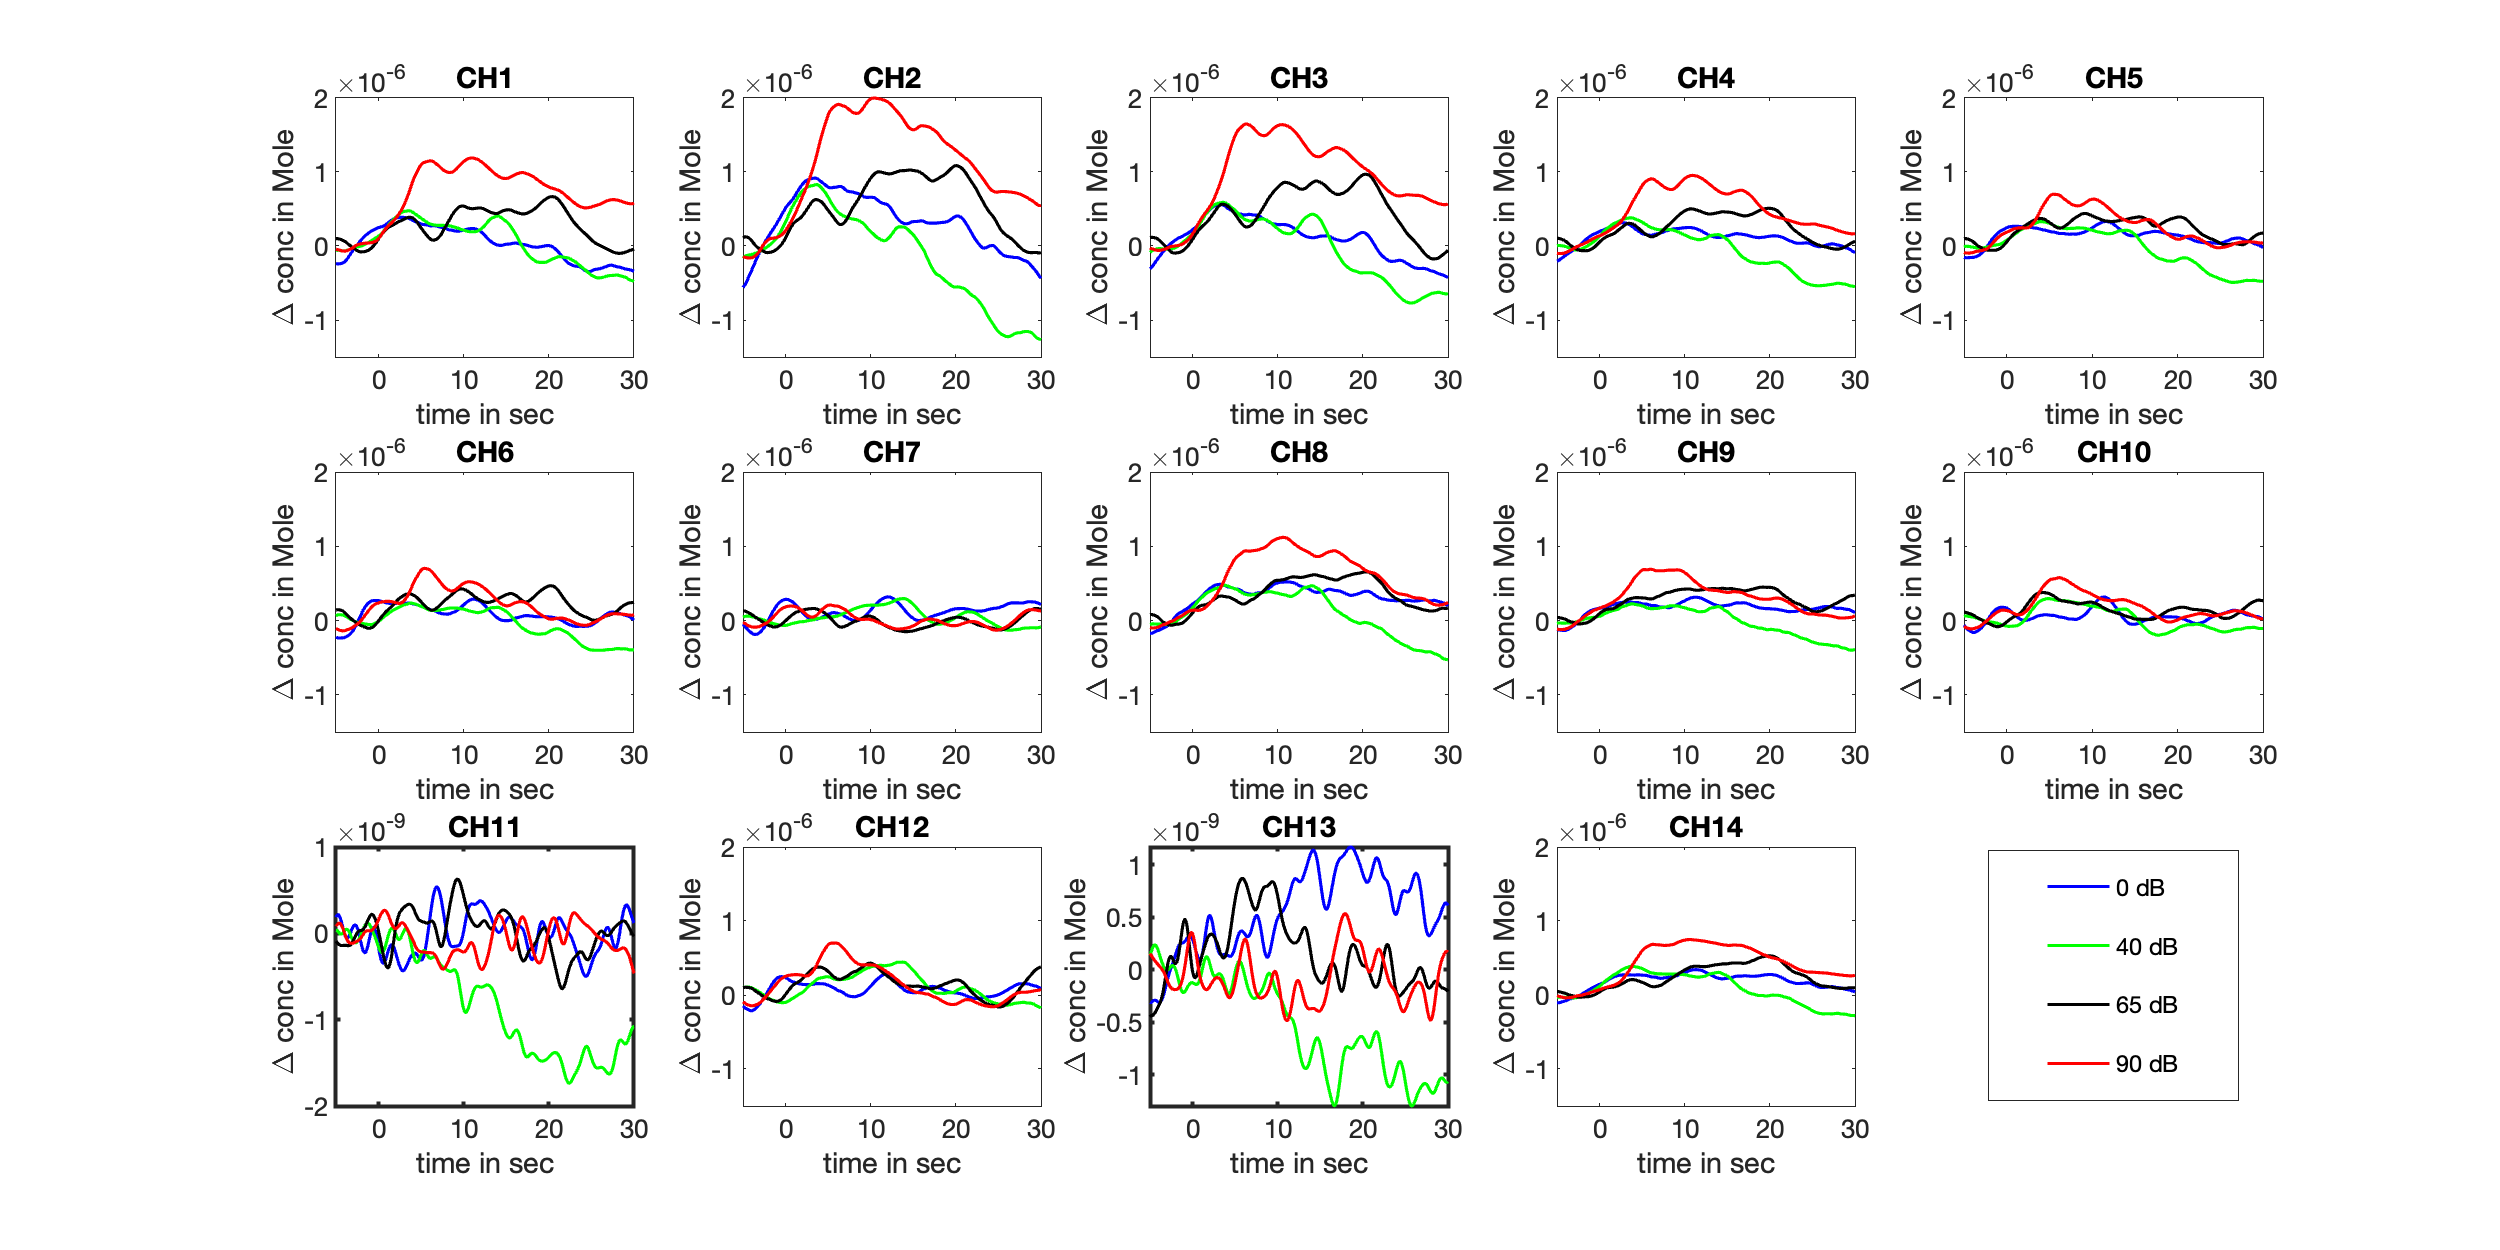
\includegraphics[scale=.4]{bilder/HbO_Mole/sub_jonas_s_HbO.png}
  \caption{Measurement from participant 3.}
  \label{fig:somesignal}
\end{figure}

\begin{figure}[H]
  \centering
    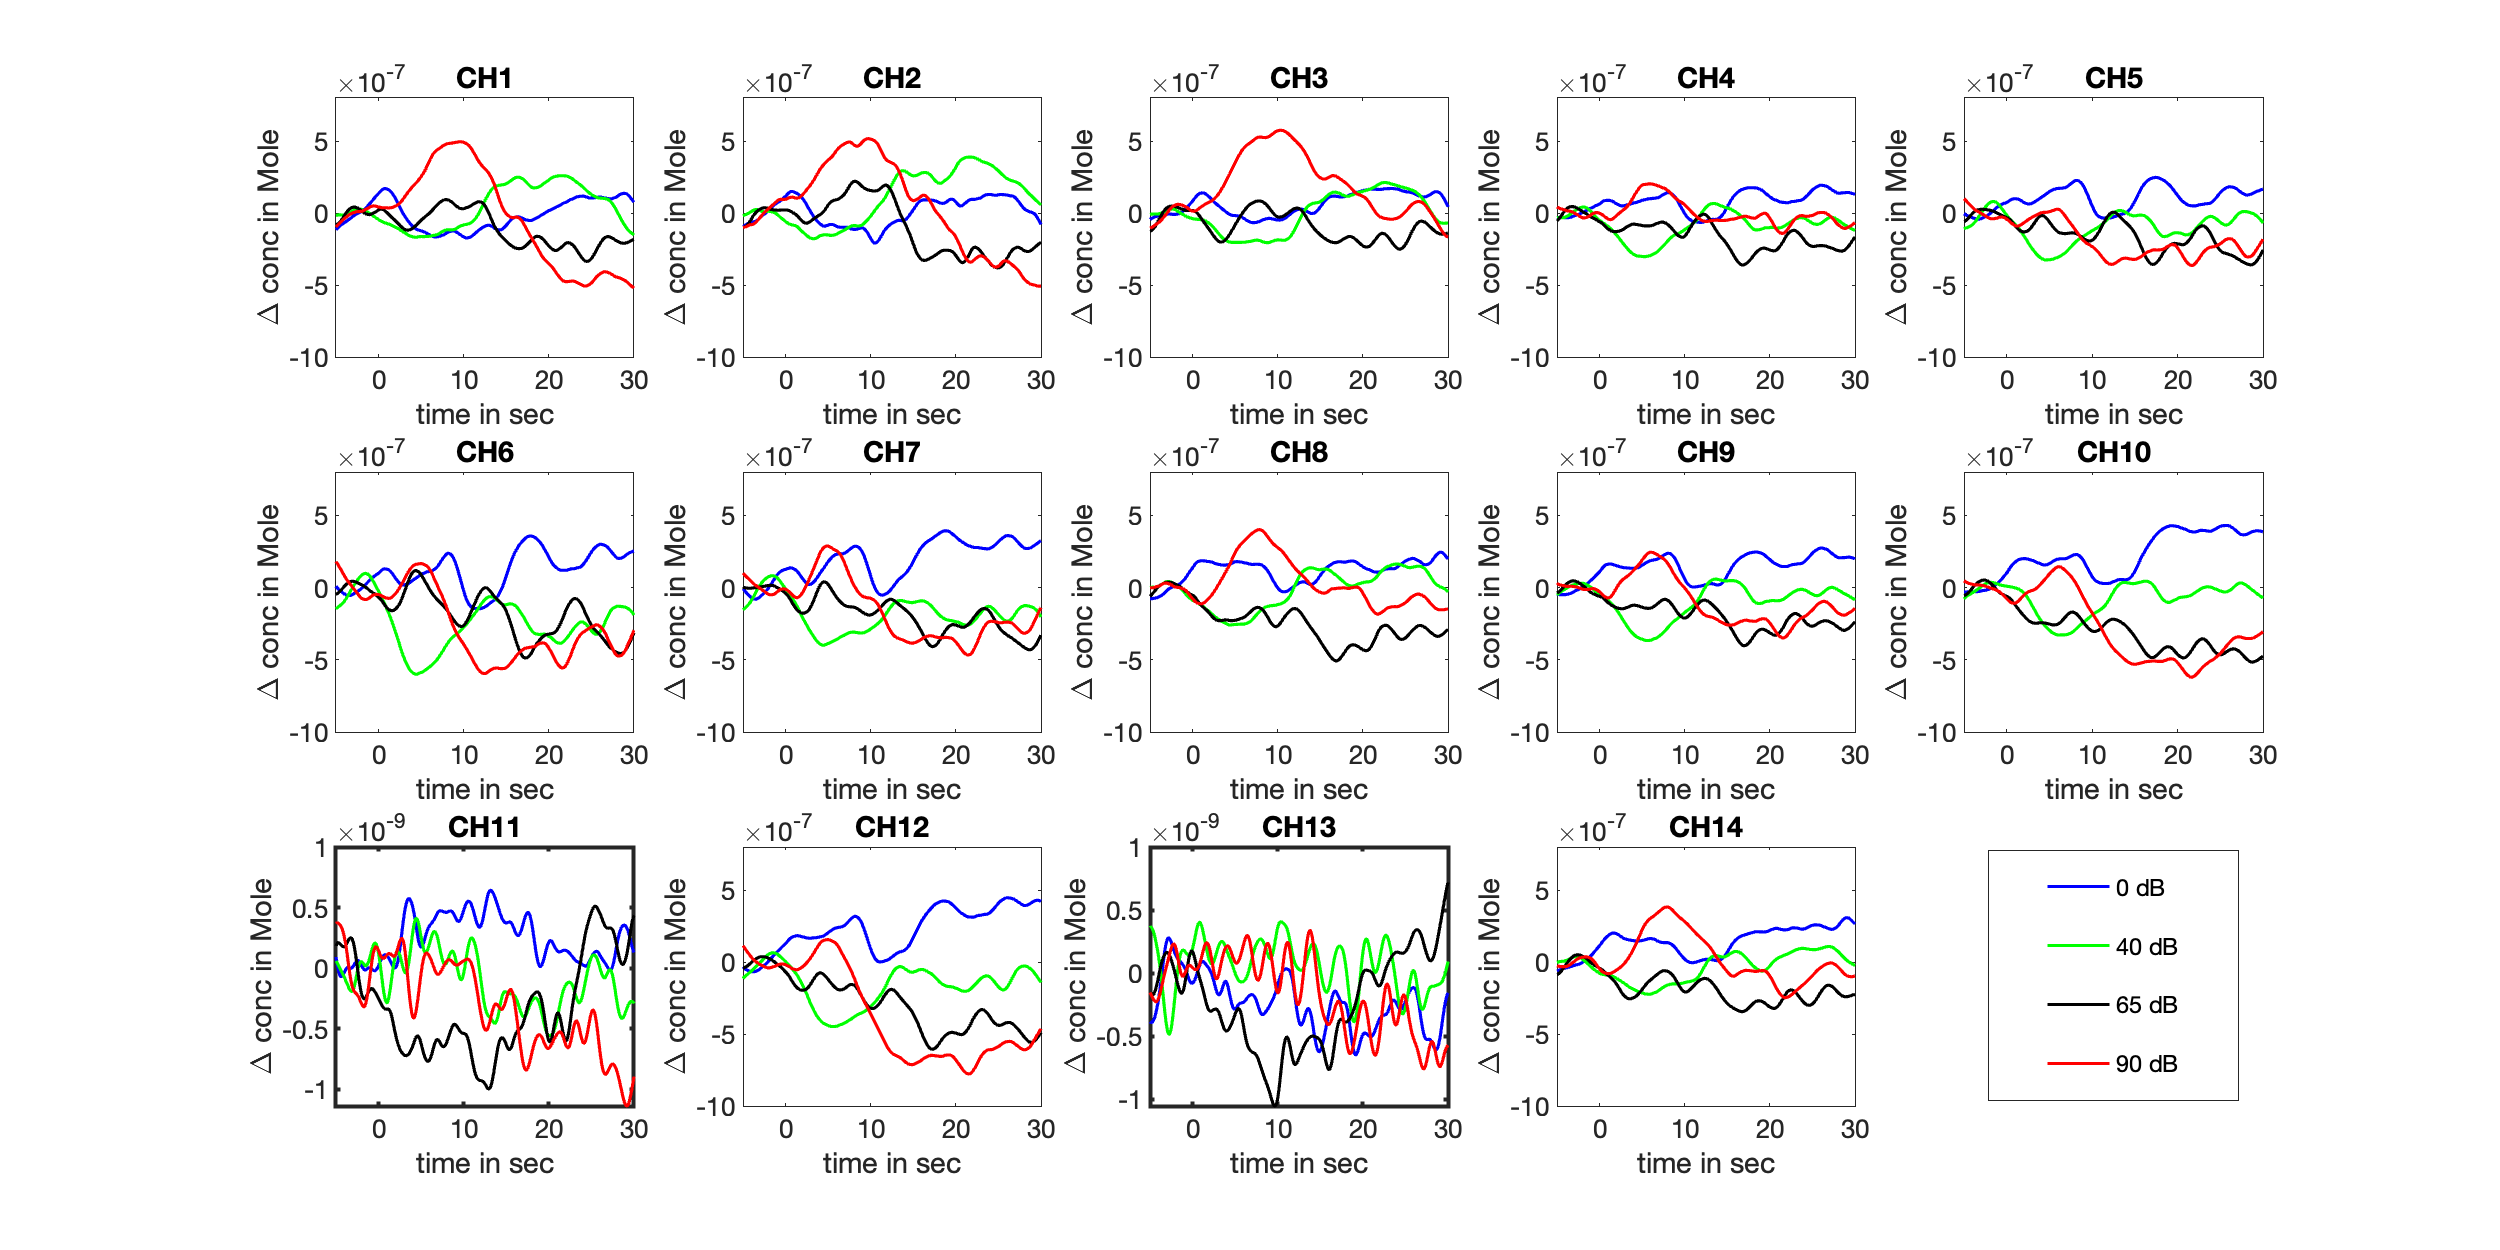
\includegraphics[scale=.4]{bilder/HbO_Mole/sub_lukas_s_HbO.png}
  \caption{Measurement from participant 5.}
  \label{fig:somesignal}
\end{figure}

\begin{figure}[H]
  \centering
    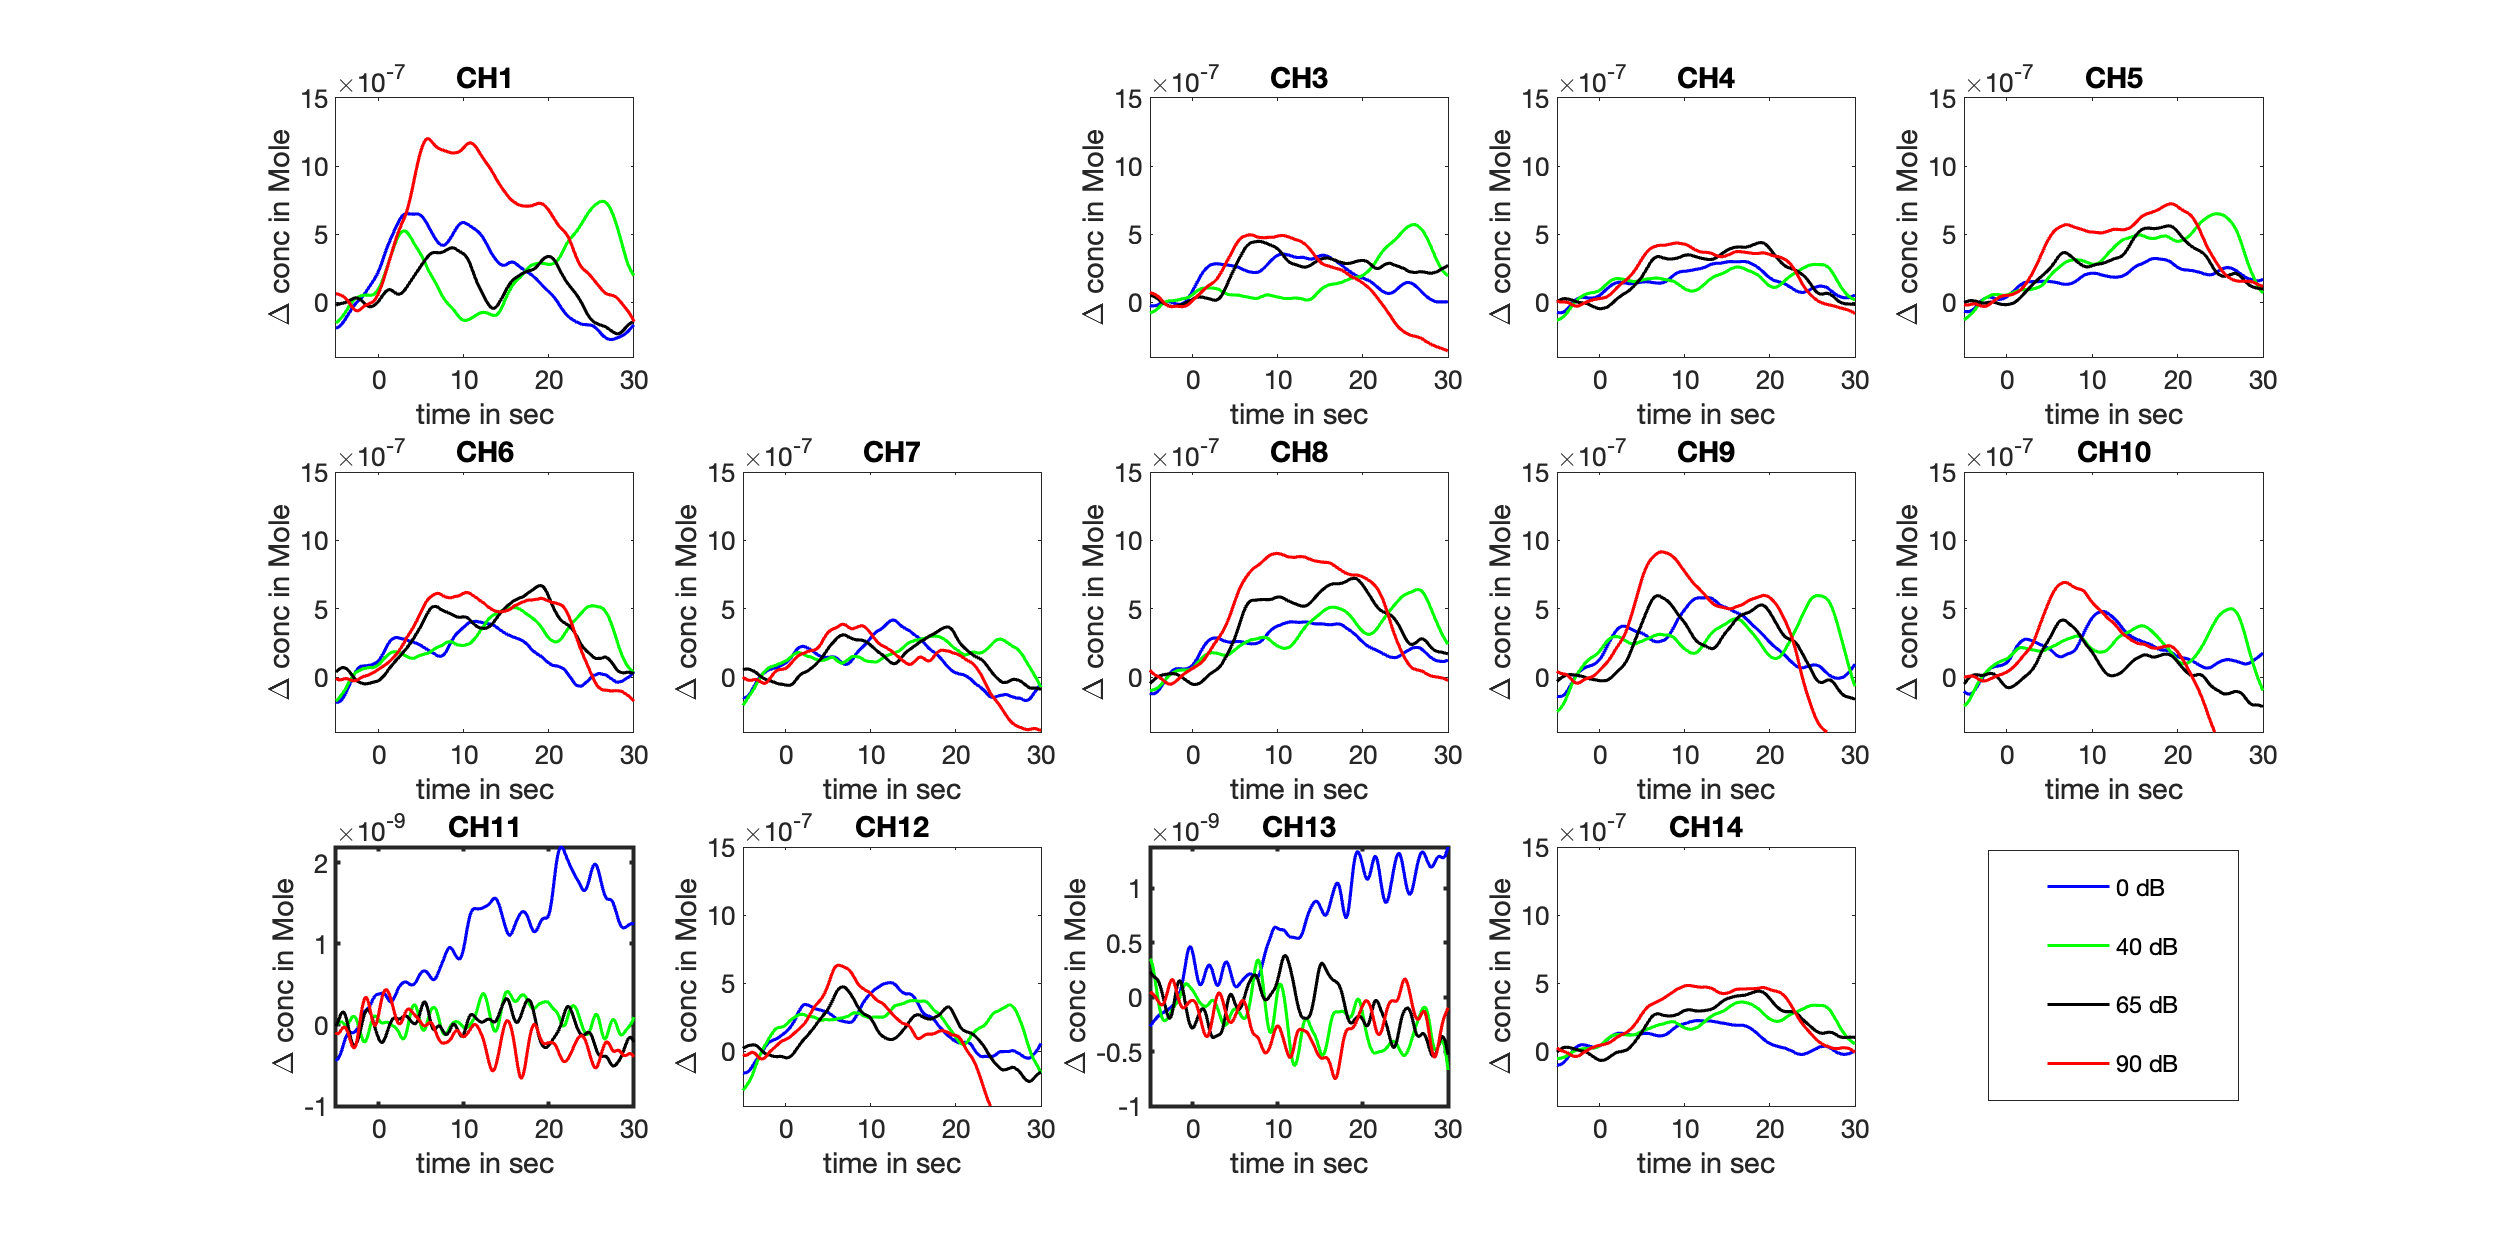
\includegraphics[scale=.4]{bilder/HbO_Mole/sub_liao_s_HbO.png}
  \caption{Measurement from participant 7.}
  \label{fig:somesignal}
\end{figure}


\begin{figure}[H]
  \centering
    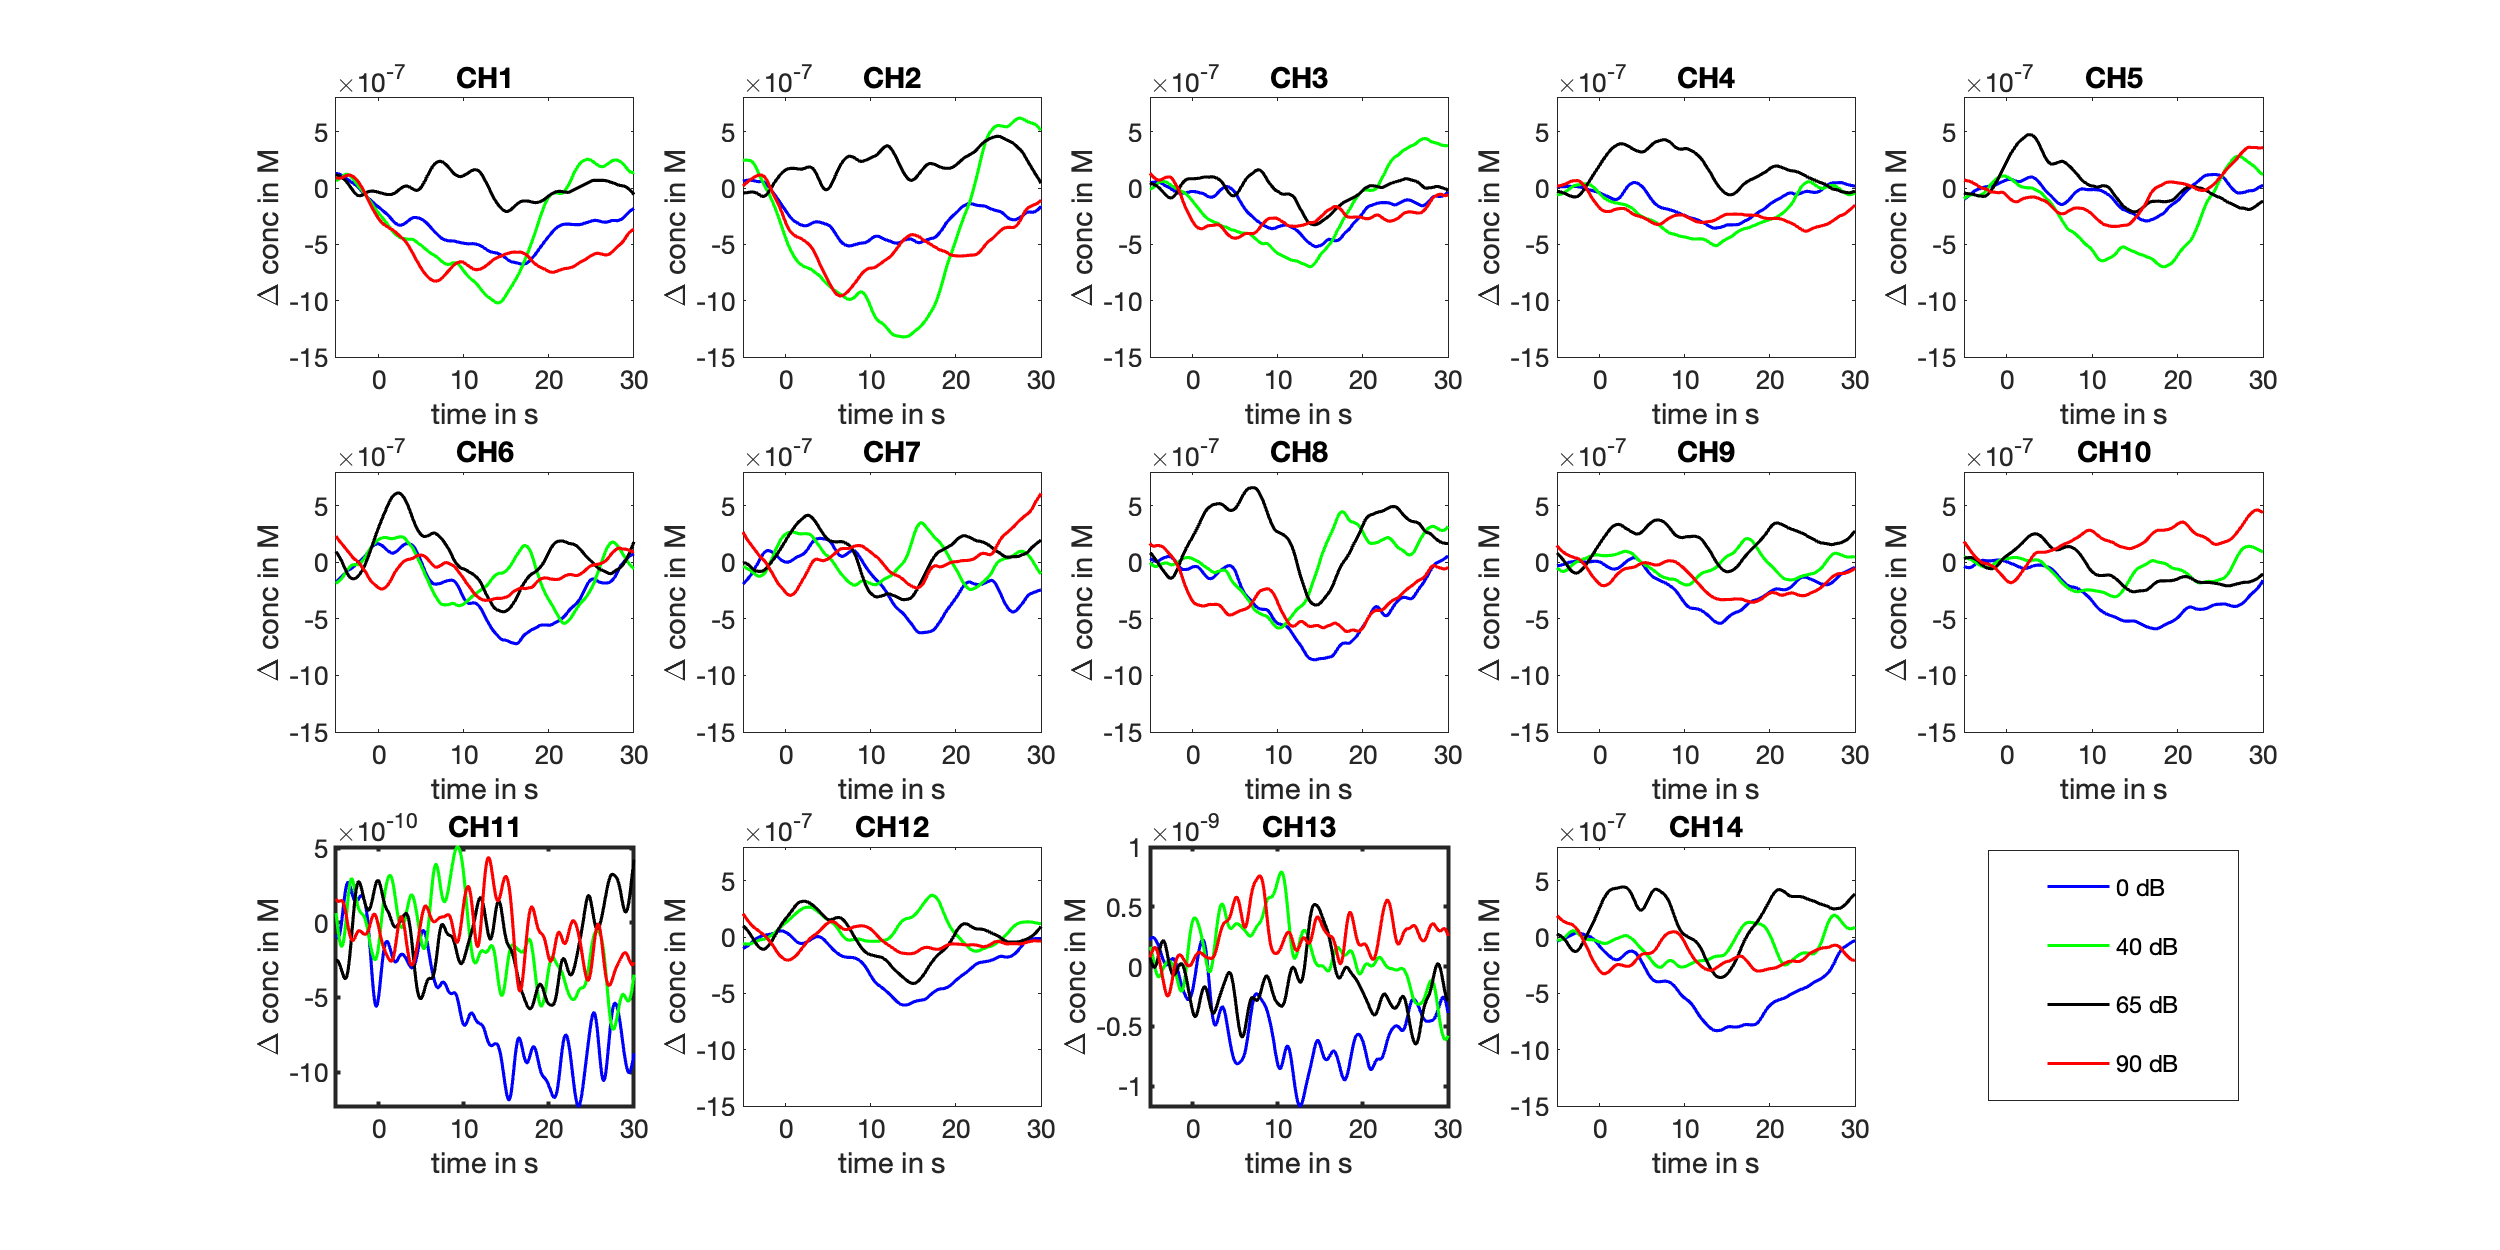
\includegraphics[scale=.4]{bilder/HbO_Mole/sub_luca2_s_HbO.png}
  \caption{Measurement from participant 8. Silent comparison}
  \label{fig:somesignal}
\end{figure}



\newpage

\subsection{Deoxygenated Hemoglobin, HbR}

\begin{figure}[H]
  \centering
    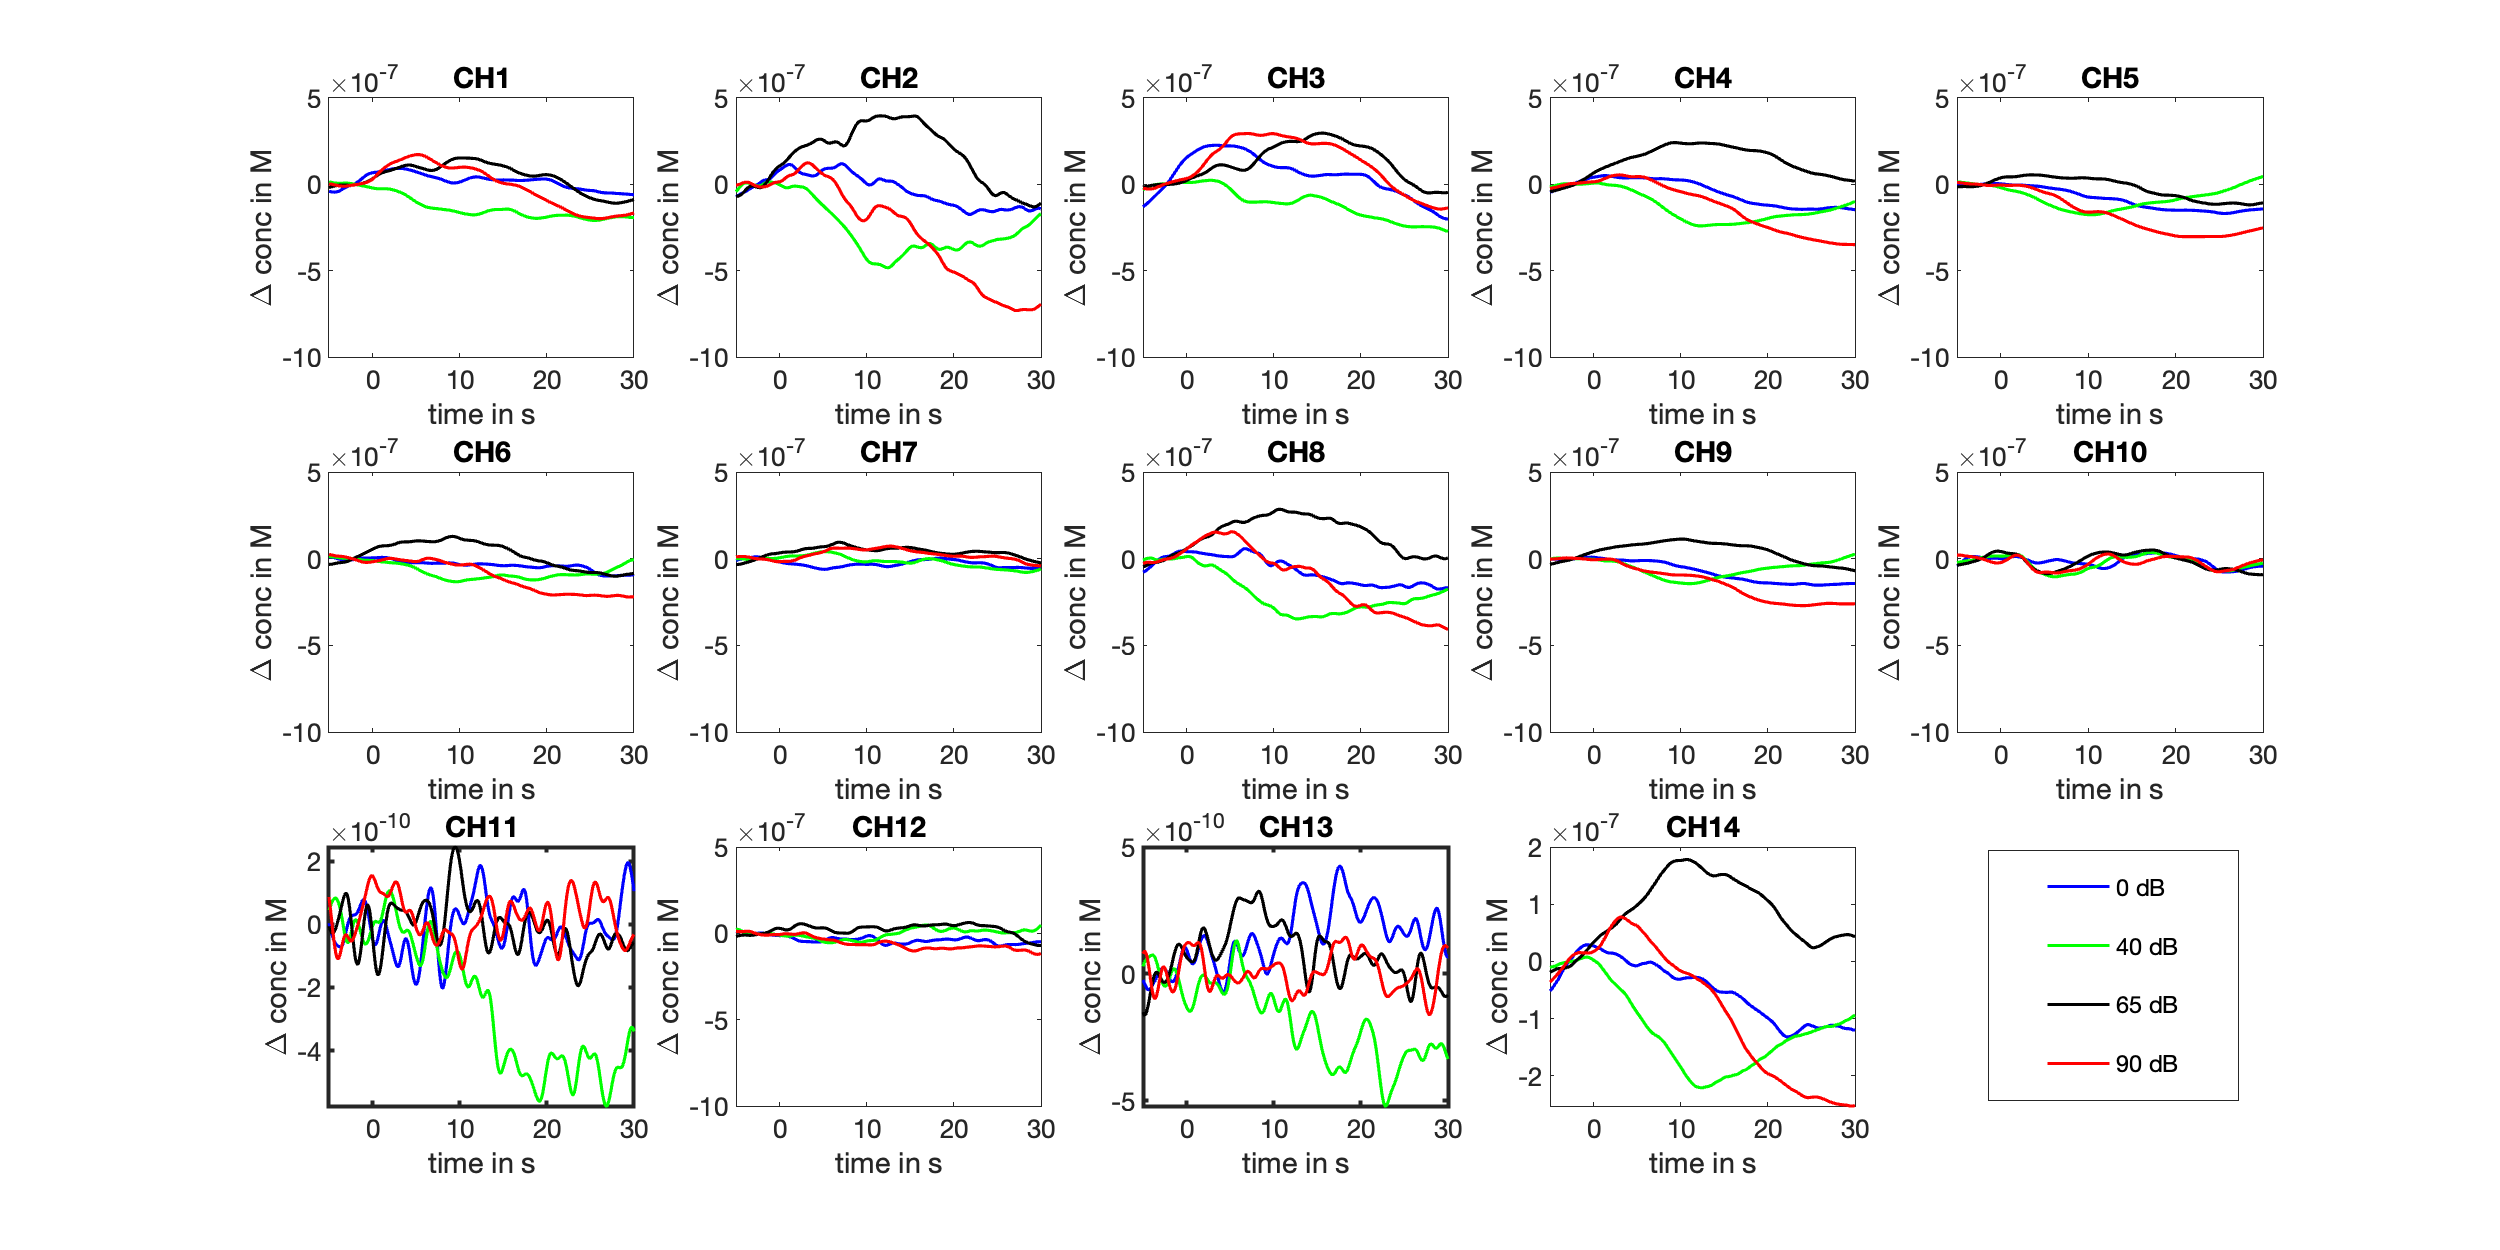
\includegraphics[scale=.4]{bilder/HbR_Mole/sub_jonas_s_HbR.png}
  \caption{Measurement from participant 3.}
  \label{fig:somesignal}
\end{figure}

\begin{figure}[H]
  \centering
    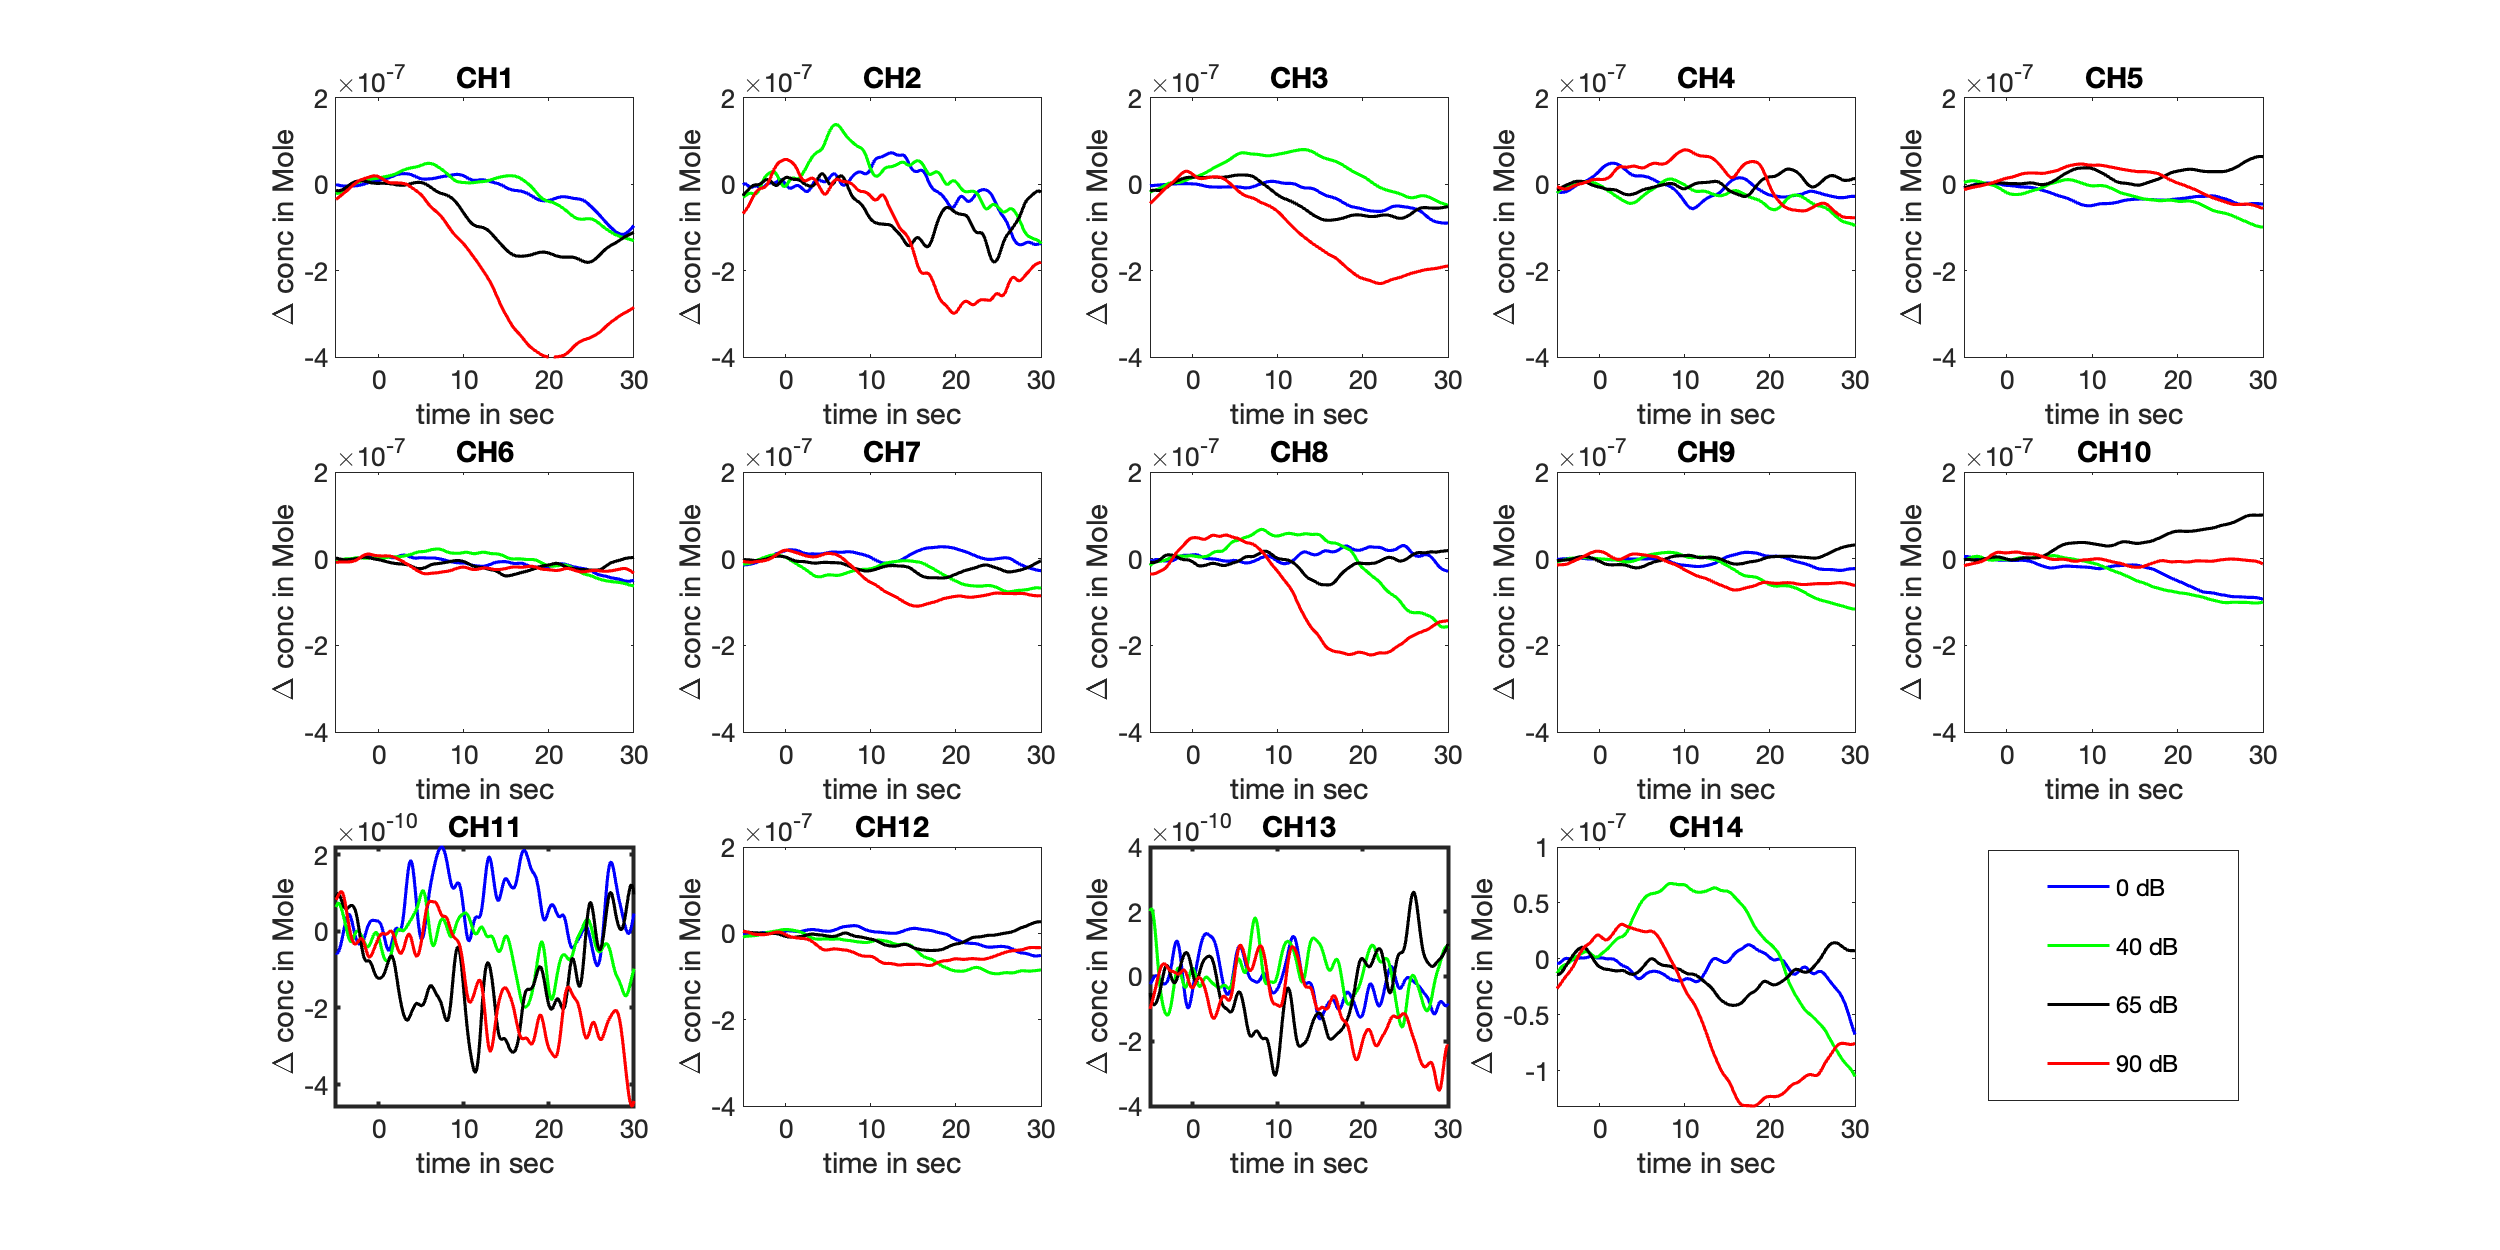
\includegraphics[scale=.4]{bilder/HbR_Mole/sub_lukas_s_HbR.png}
  \caption{Measurement from participant 5.}
  \label{fig:somesignal}
\end{figure}

\begin{figure}[H]
  \centering
    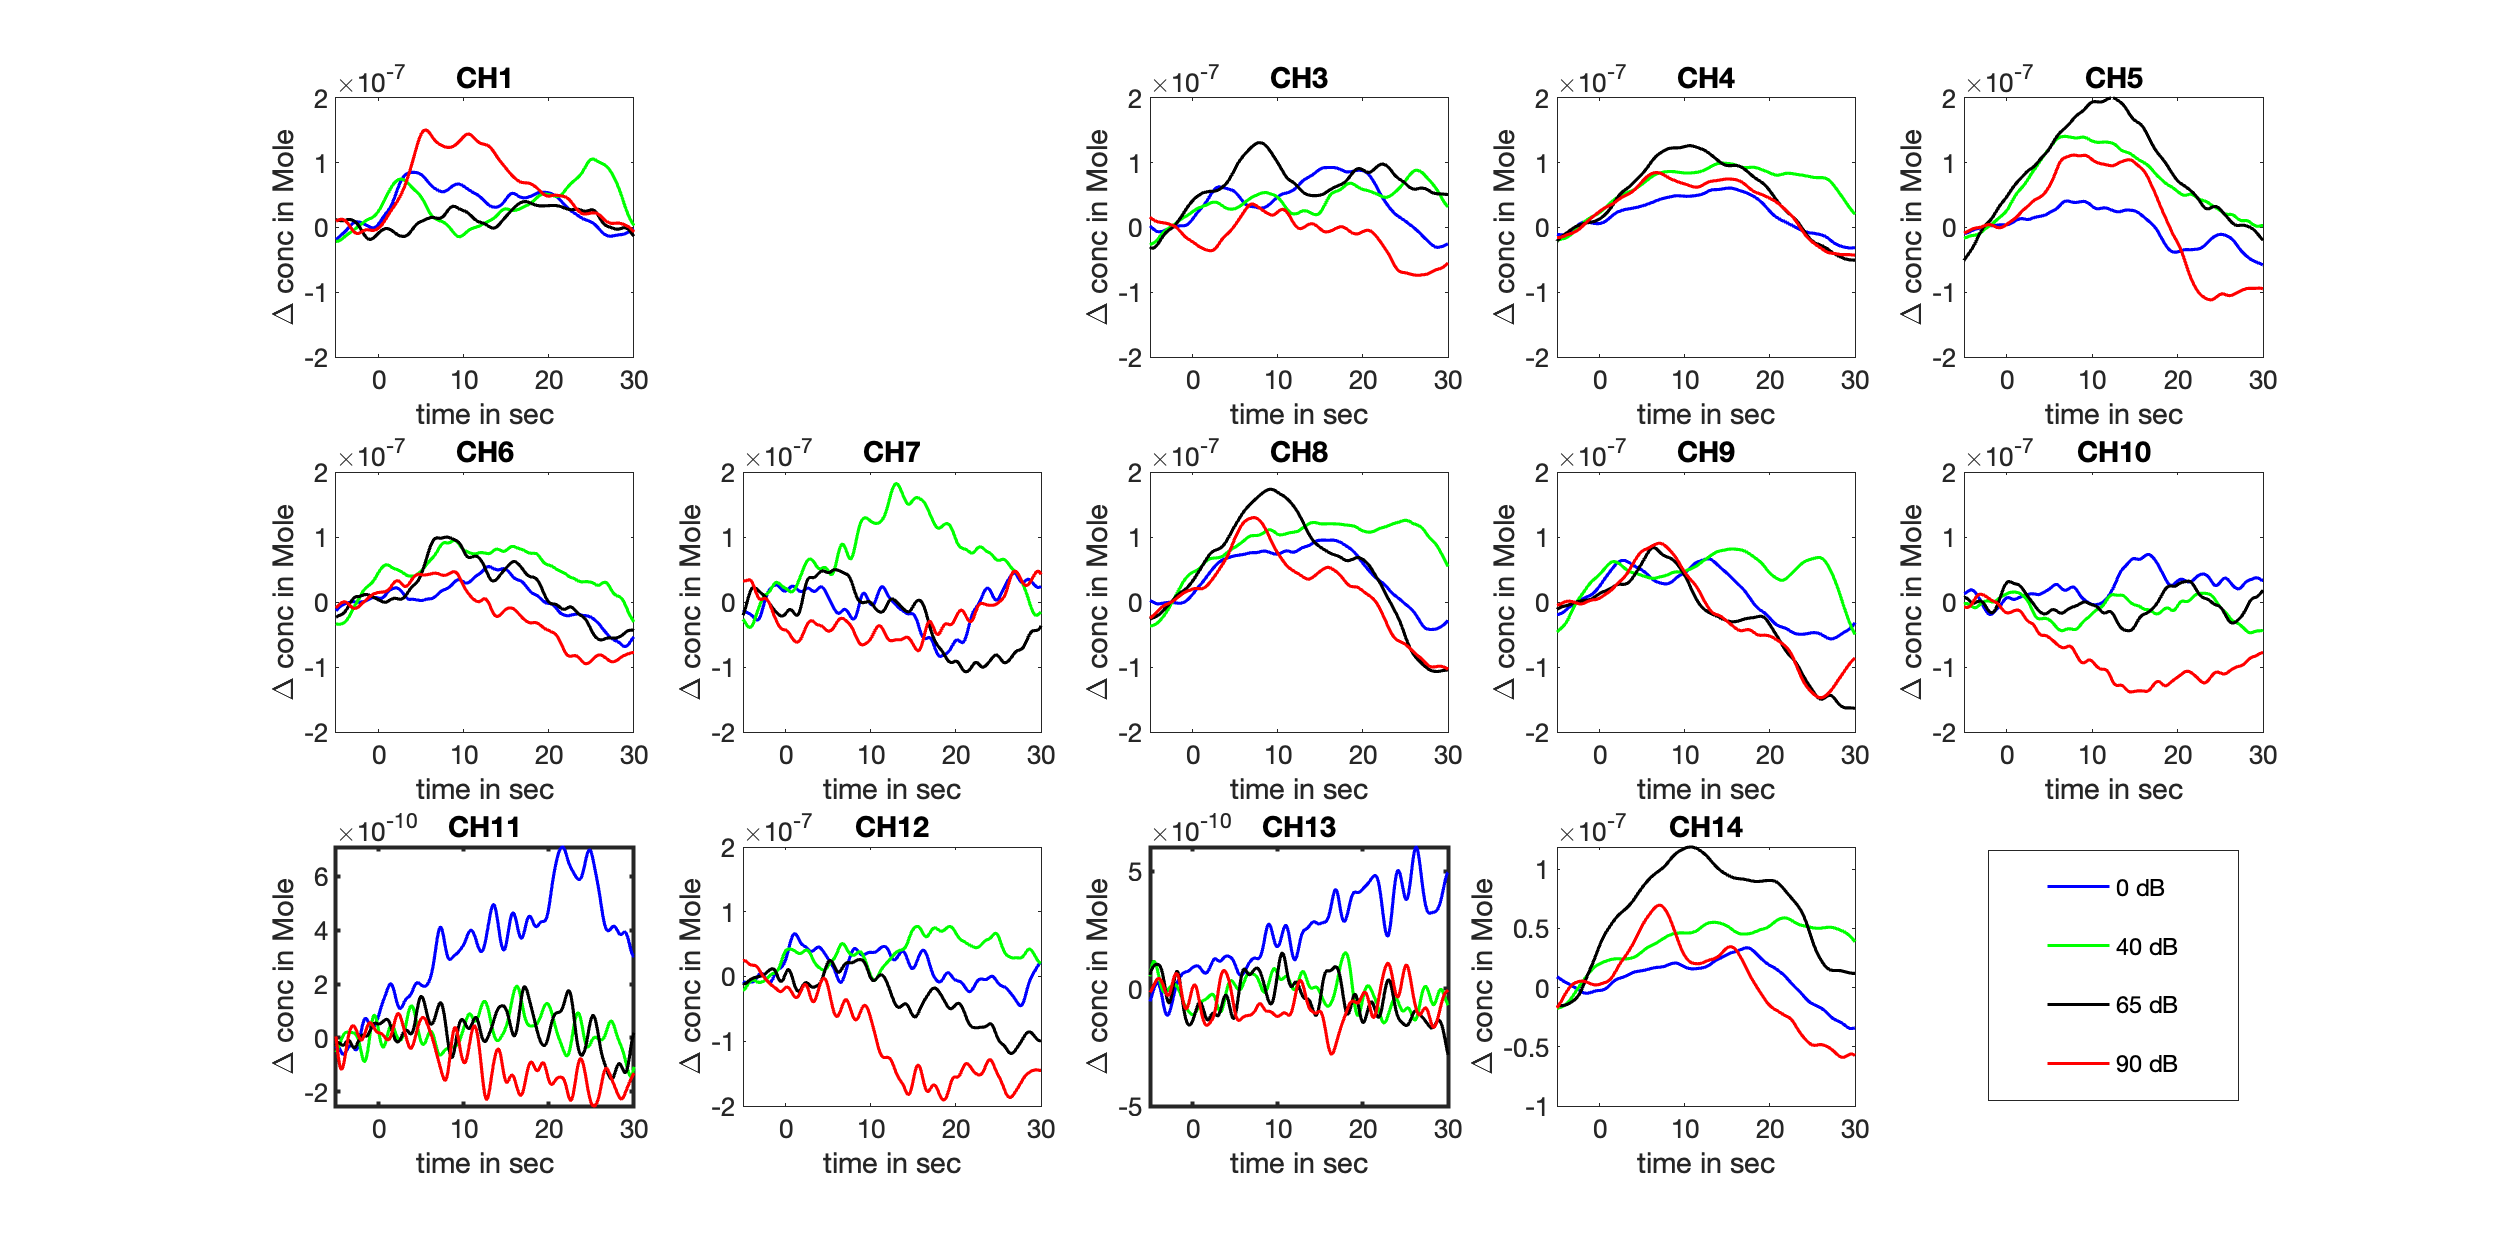
\includegraphics[scale=.4]{bilder/HbR_Mole/sub_liao_s_HbR.png}
  \caption{Measurement from participant 7.}
  \label{fig:somesignal}
\end{figure}


\begin{figure}[H]
  \centering
    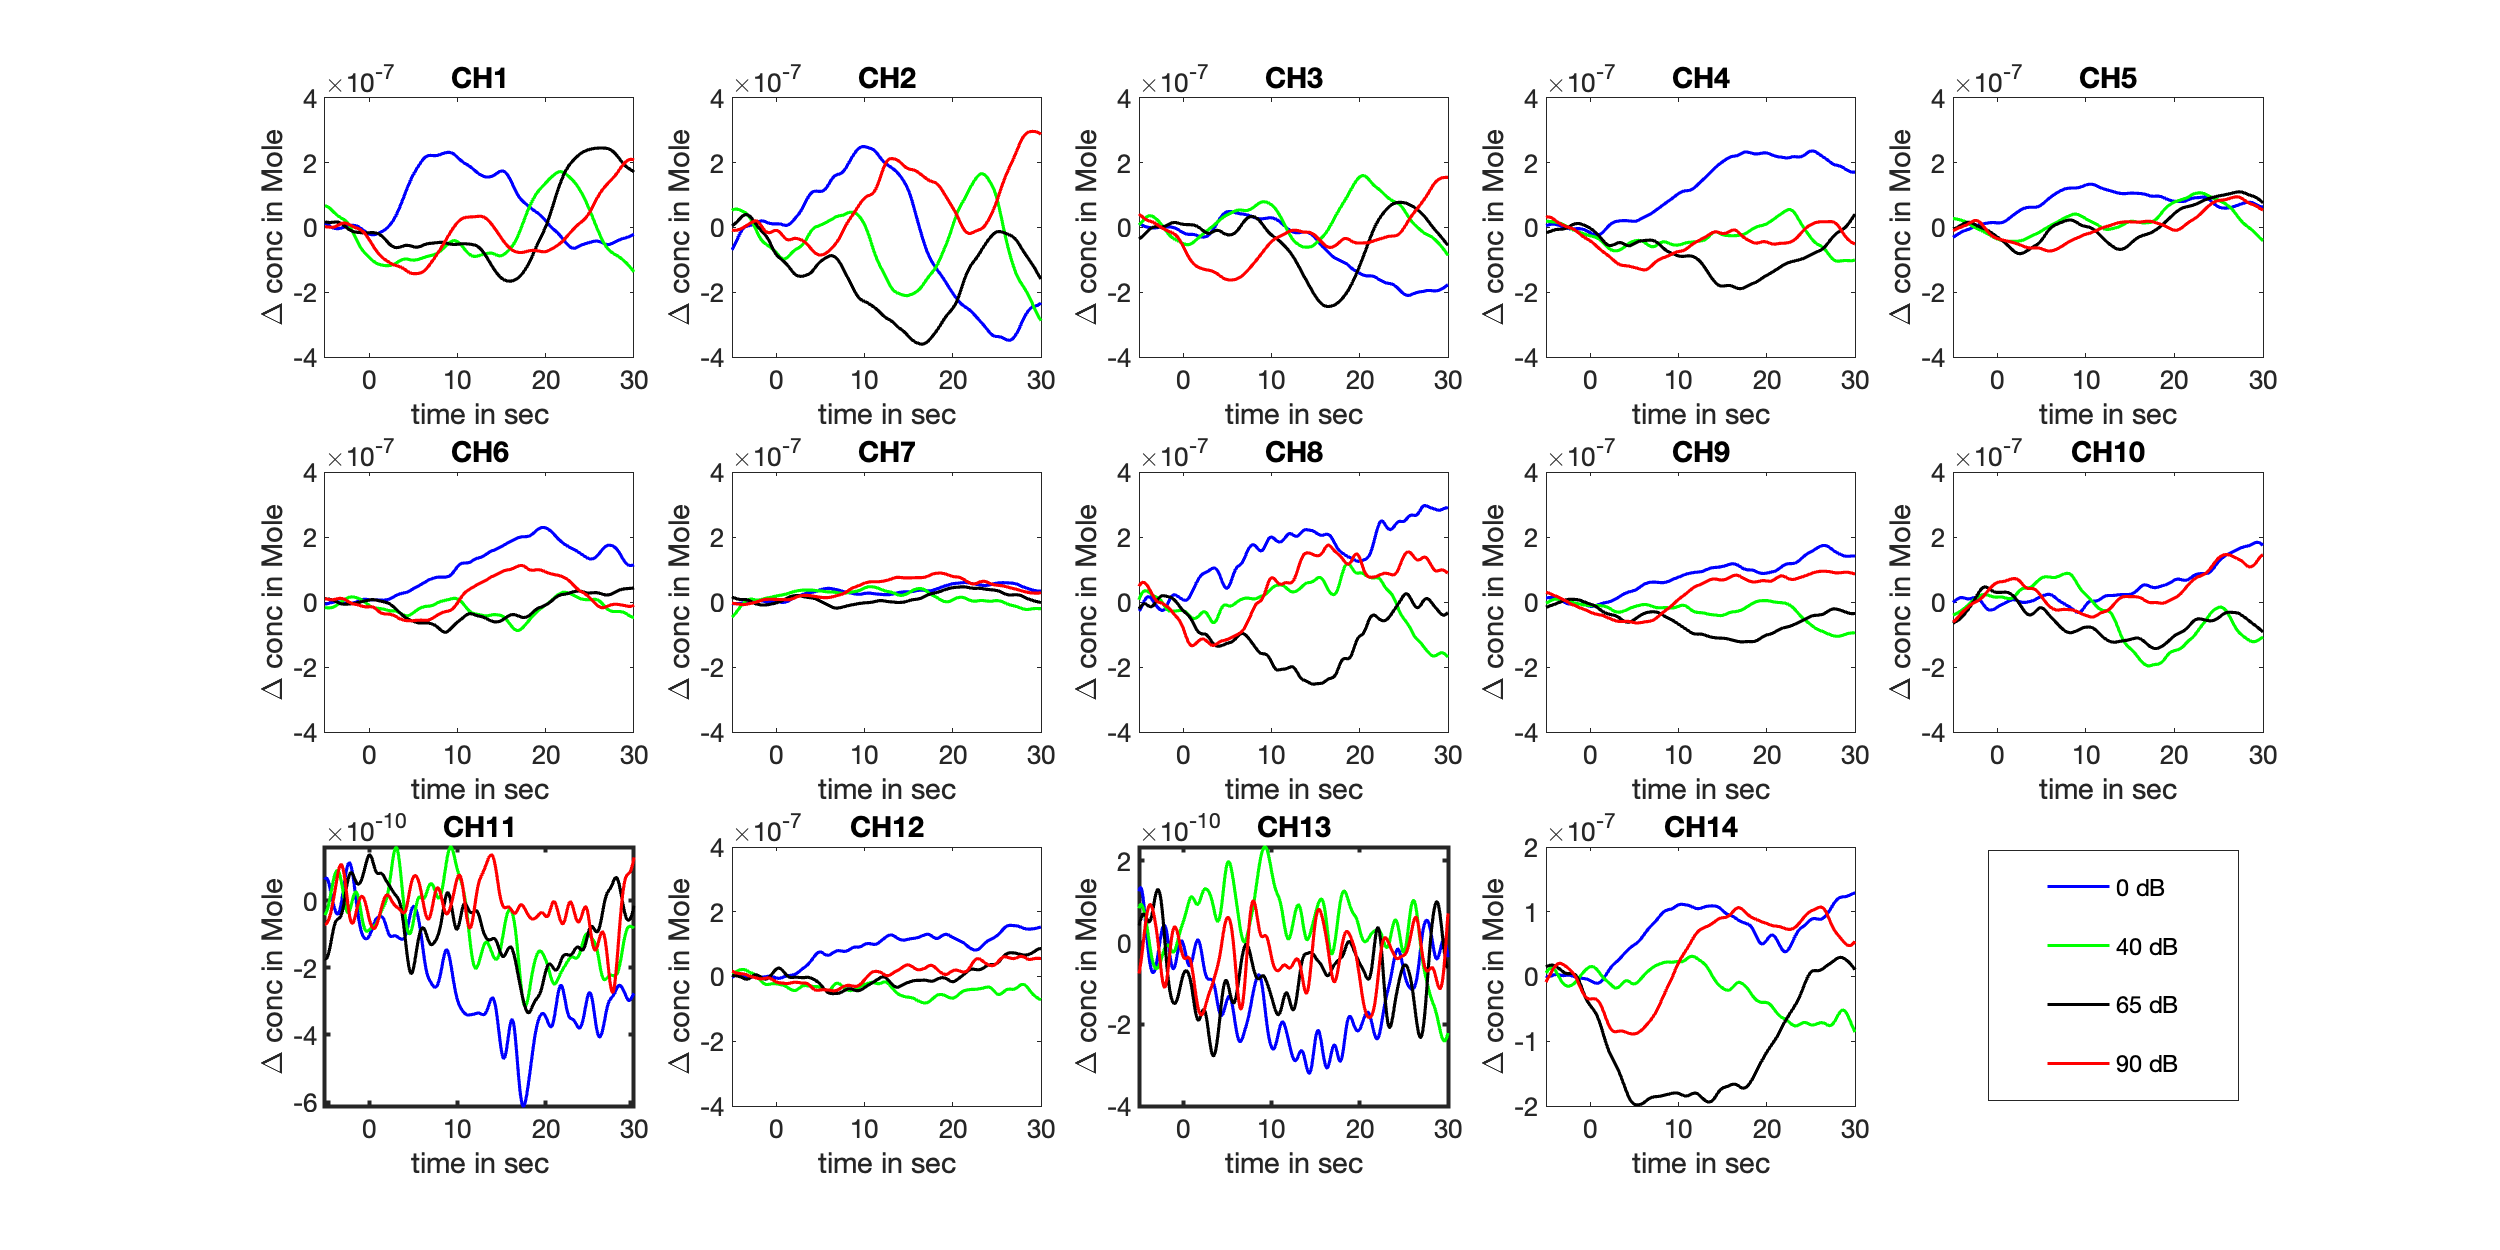
\includegraphics[scale=.4]{bilder/HbR_Mole/sub_luca2_s_HbR.png}
  \caption{Measurement from participant 8. Silent comparison}
  \label{fig:somesignal}
\end{figure}





\section {Region of Interest}
In the following, regions of interest is defined as [picture to be added]. The following figures shows the averaged response of all the valid channels in the defined region.
\begin{figure}[H]
  \centering
    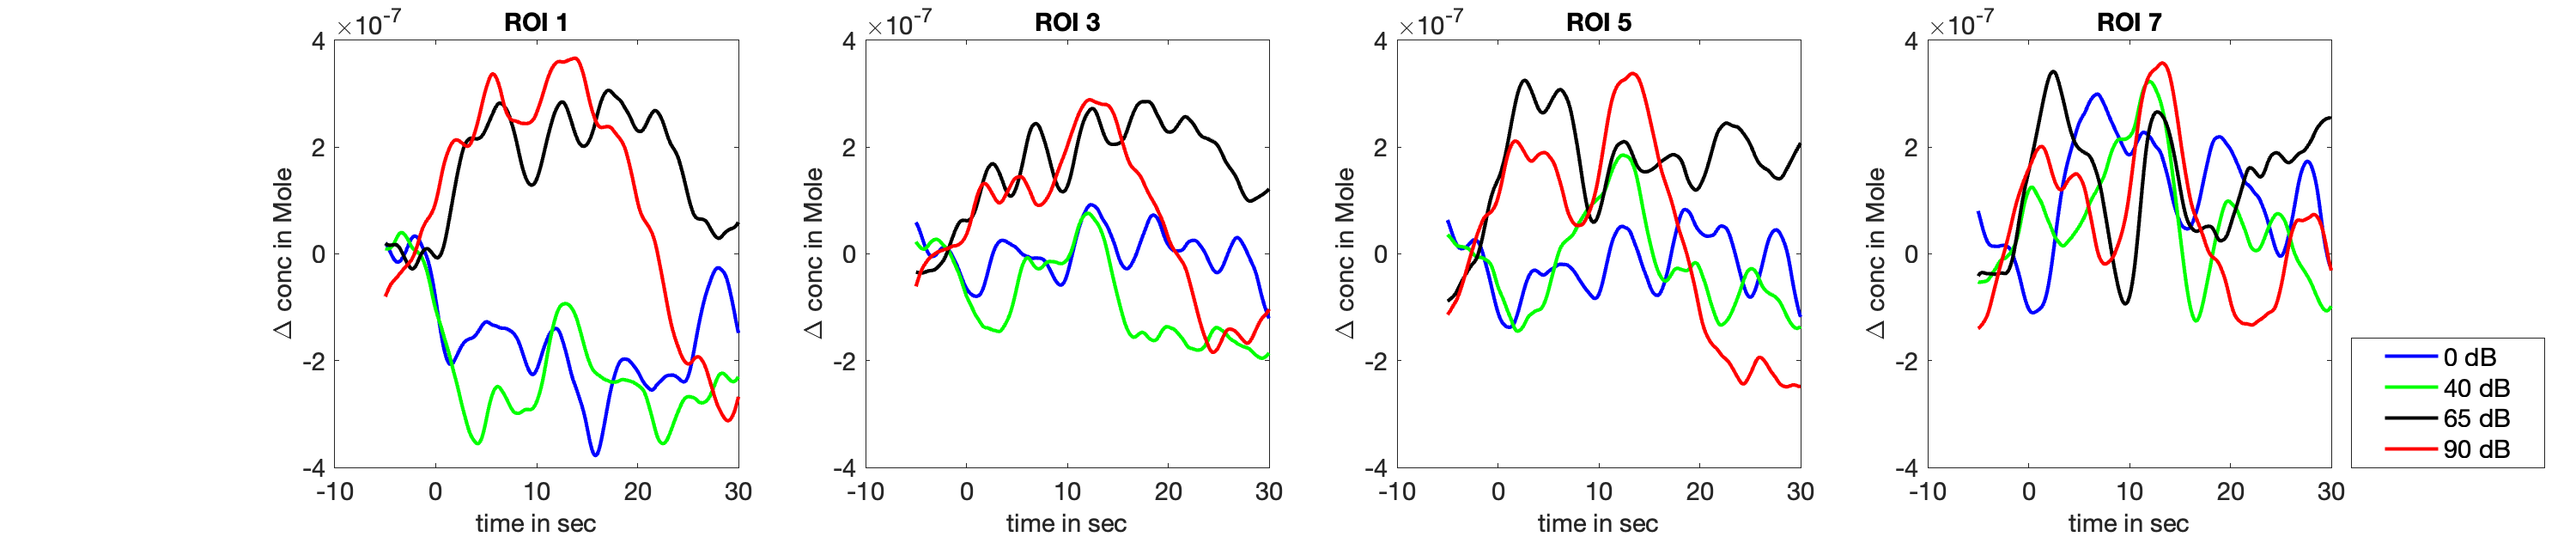
\includegraphics[scale=.29]{bilder/ROI/sub_chang_s_HbO.png}
  \caption{Measurement from participant  1.}
  \label{fig:somesignal}
\end{figure}

\begin{figure}[H]
  \centering
    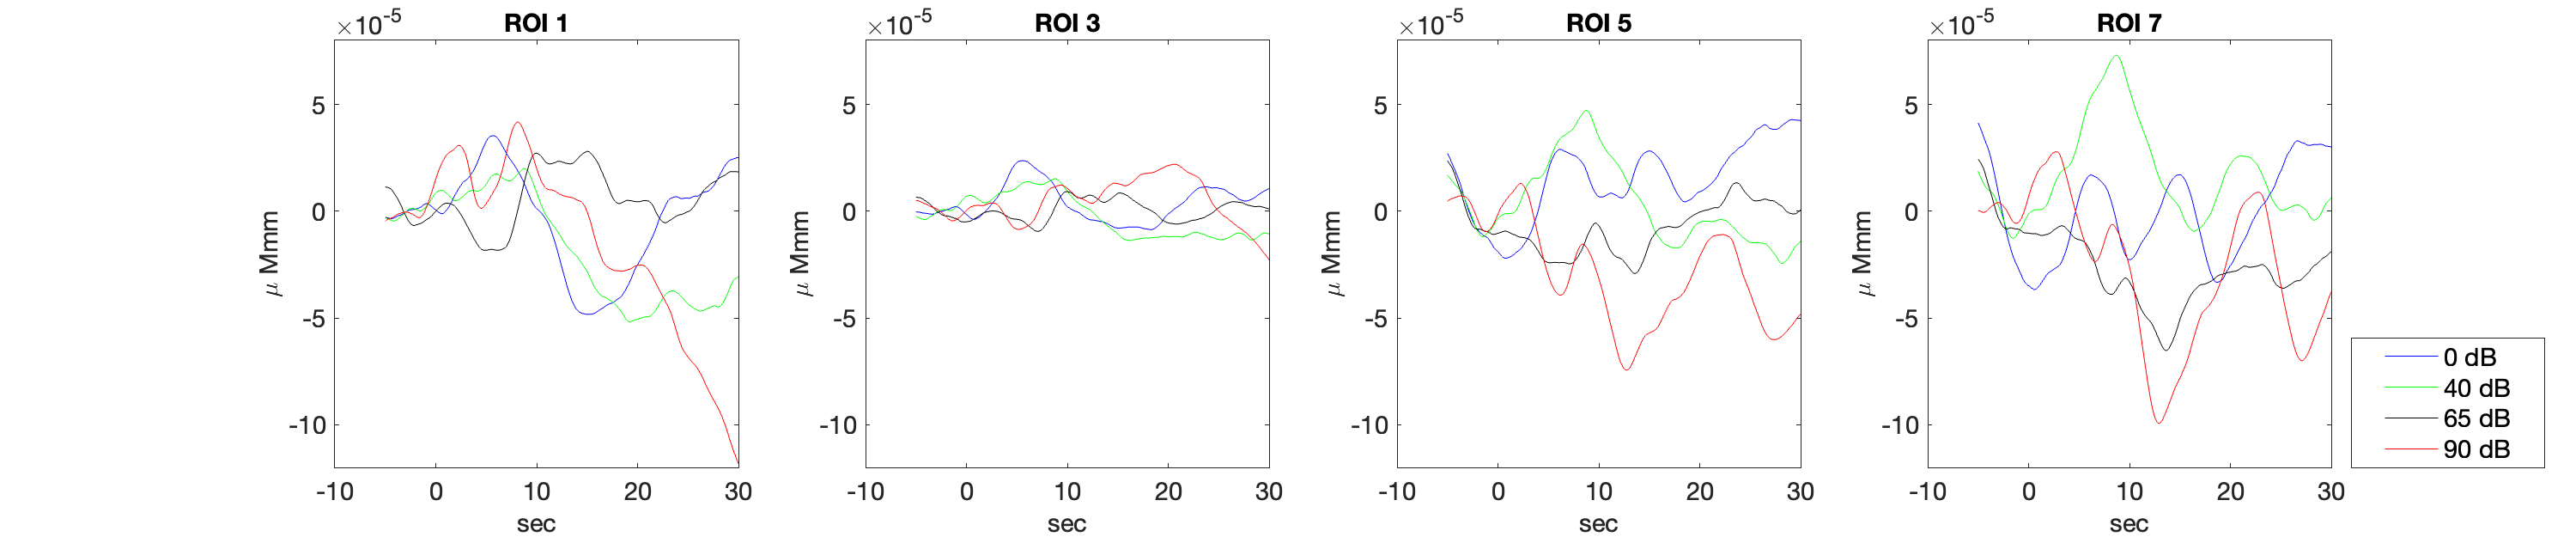
\includegraphics[scale=.29]{bilder/ROI/sub_gleb2_s_HbO.png}
  \caption{Measurement from participant  2.}
  \label{fig:somesignal}
\end{figure}

\begin{figure}[H]
  \centering
    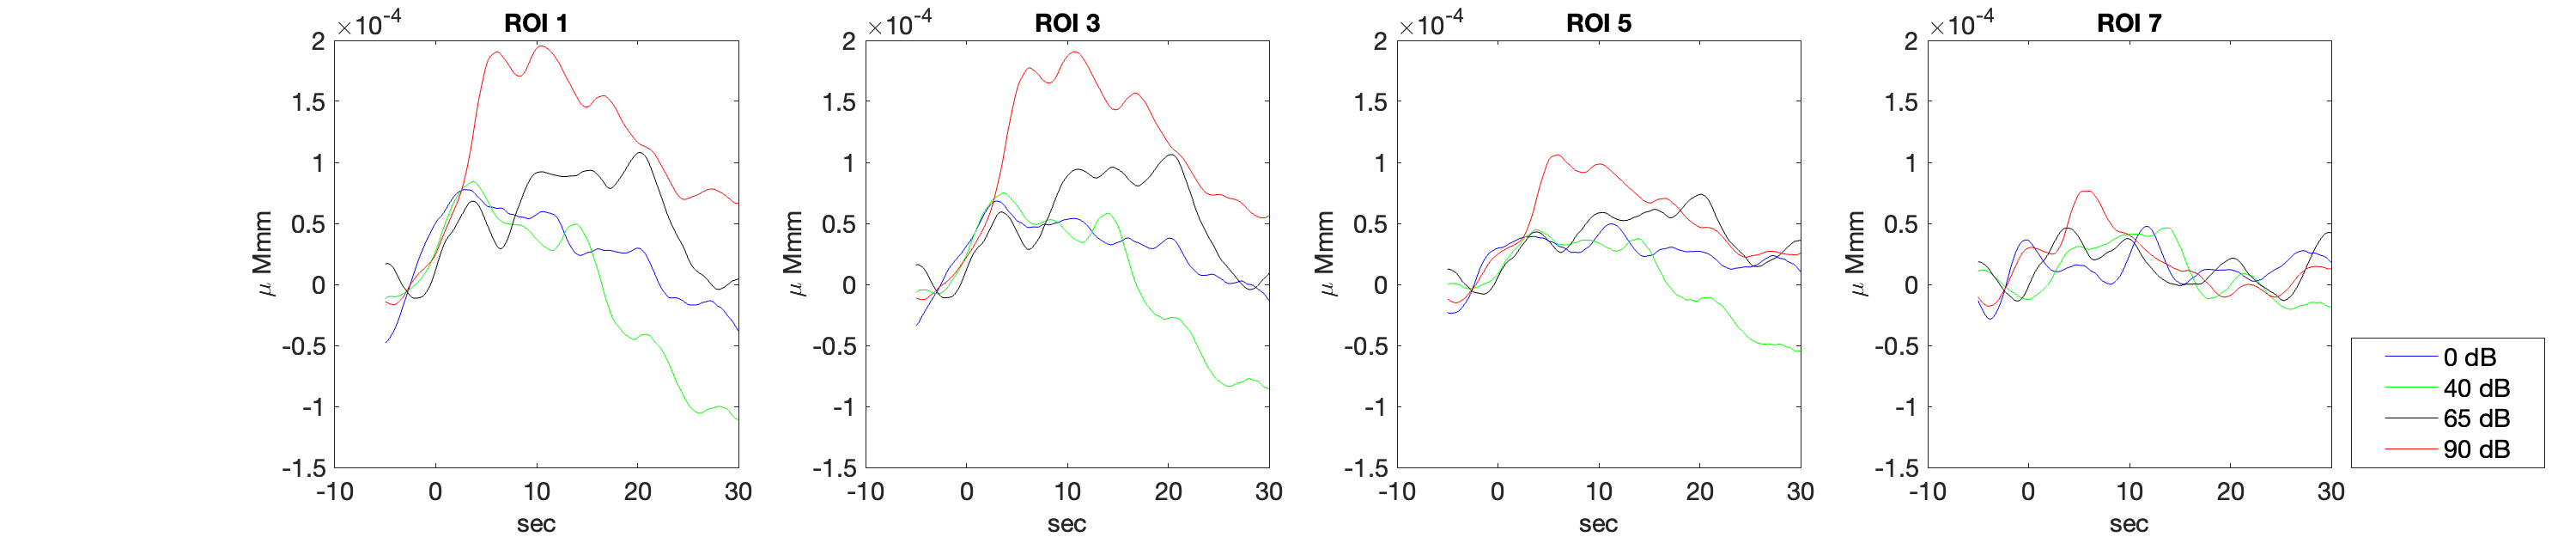
\includegraphics[scale=.29]{bilder/ROI/sub_jonas_s_HbO.png}
  \caption{Measurement from participant  3.}
  \label{fig:somesignal}
\end{figure}

\begin{figure}[H]
  \centering
    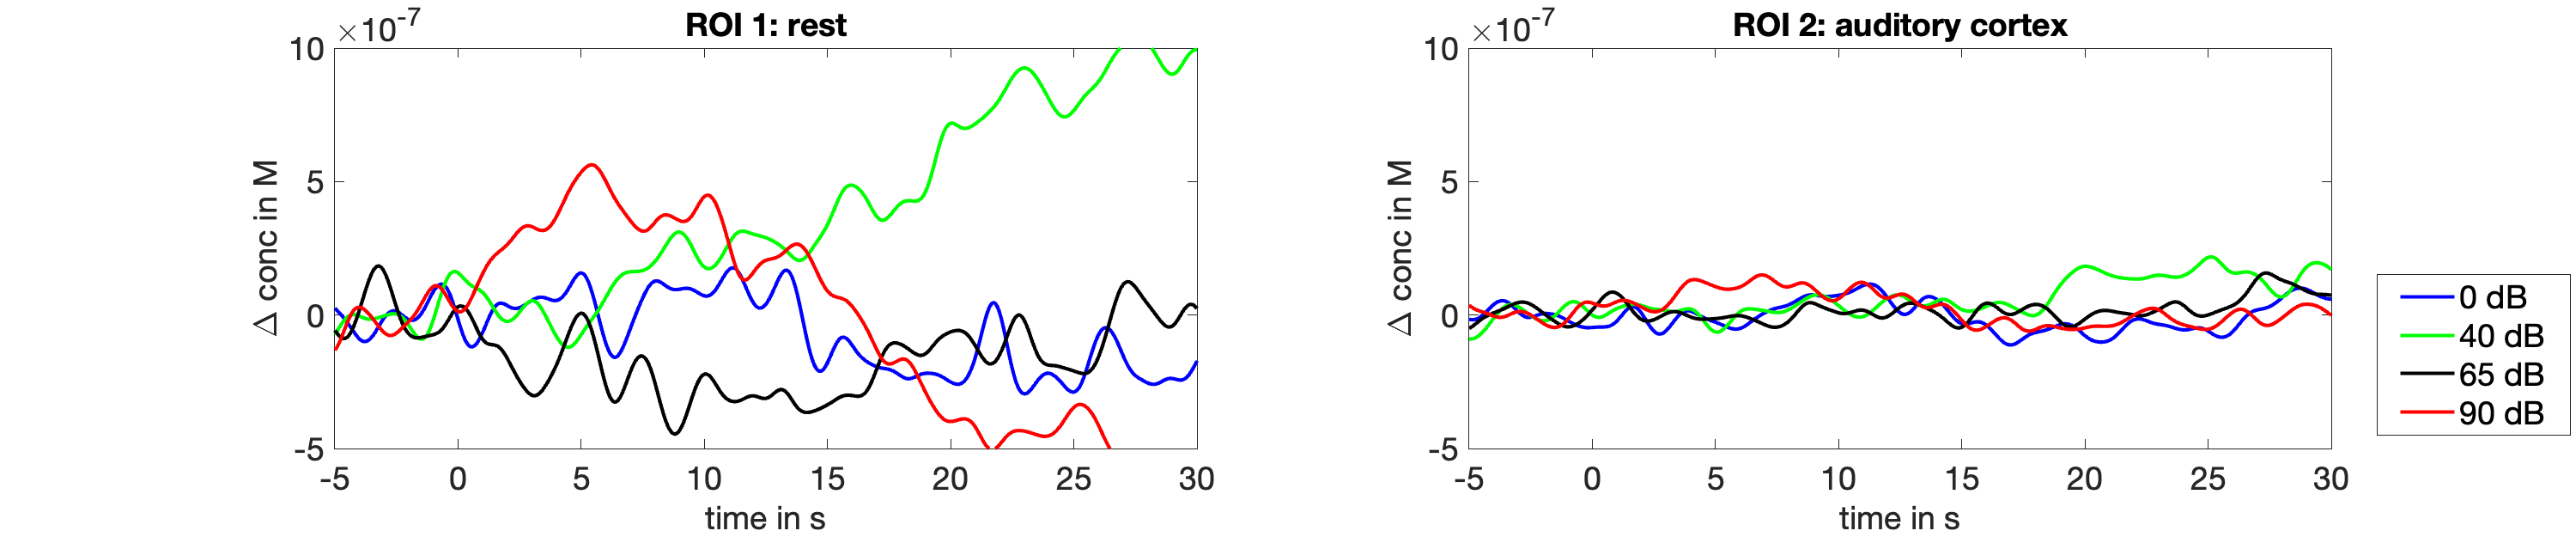
\includegraphics[scale=.29]{bilder/ROI/sub_lin_s_HbO.png}
  \caption{Measurement from participant  4.}
  \label{fig:somesignal}
\end{figure}

\begin{figure}[H]
  \centering
    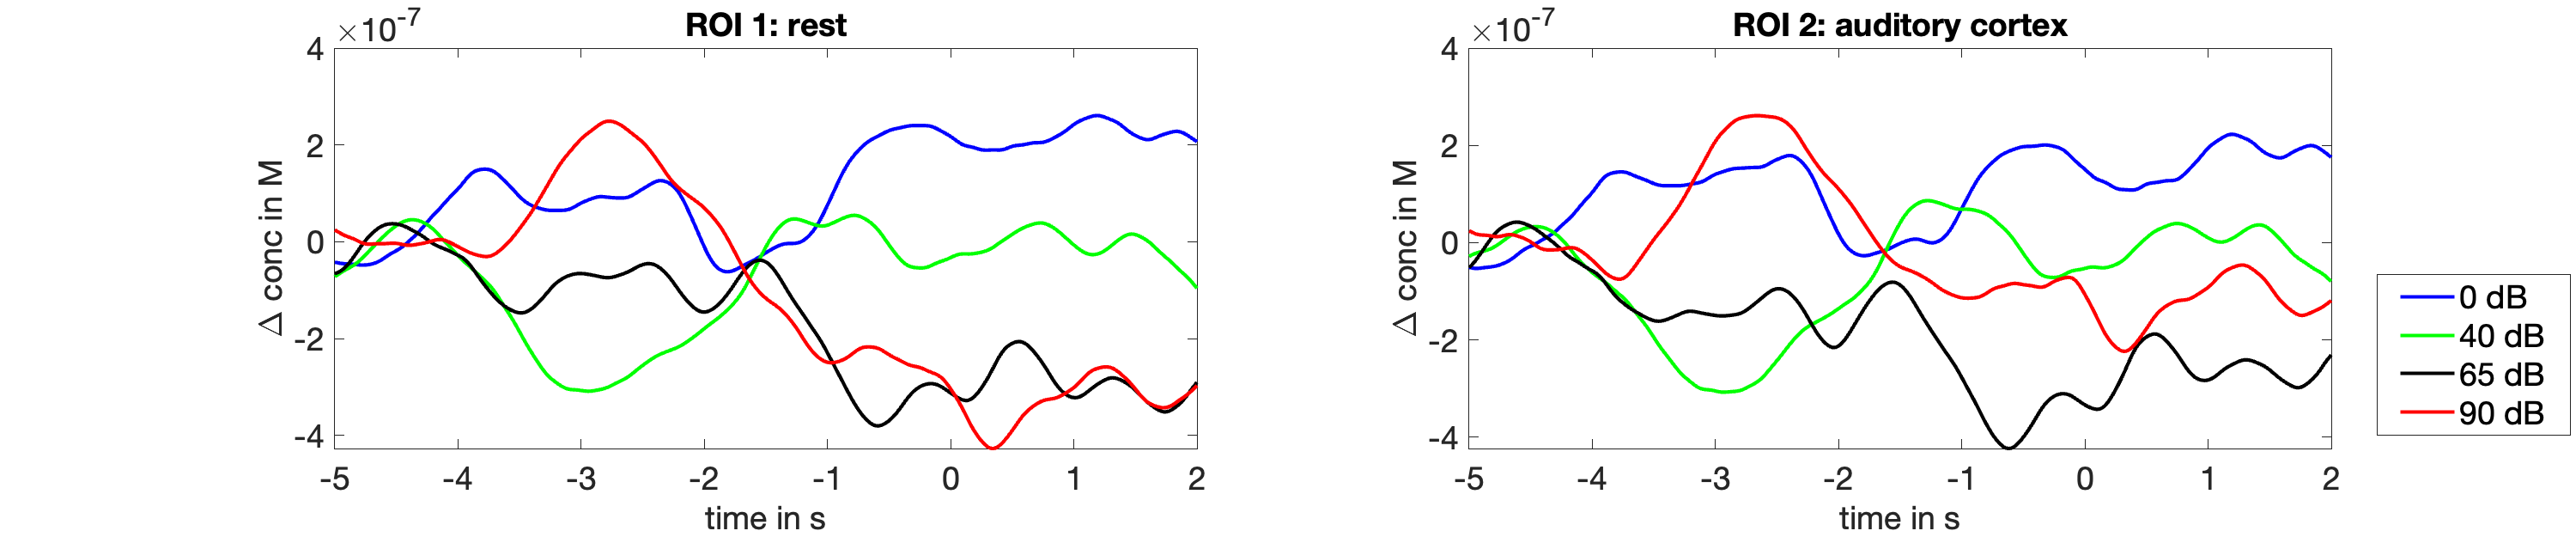
\includegraphics[scale=.29]{bilder/ROI/sub_lukas_s_HbO.png}
  \caption{Measurement from participant 5.}
  \label{fig:somesignal}
\end{figure}

\begin{figure}[H]
  \centering
    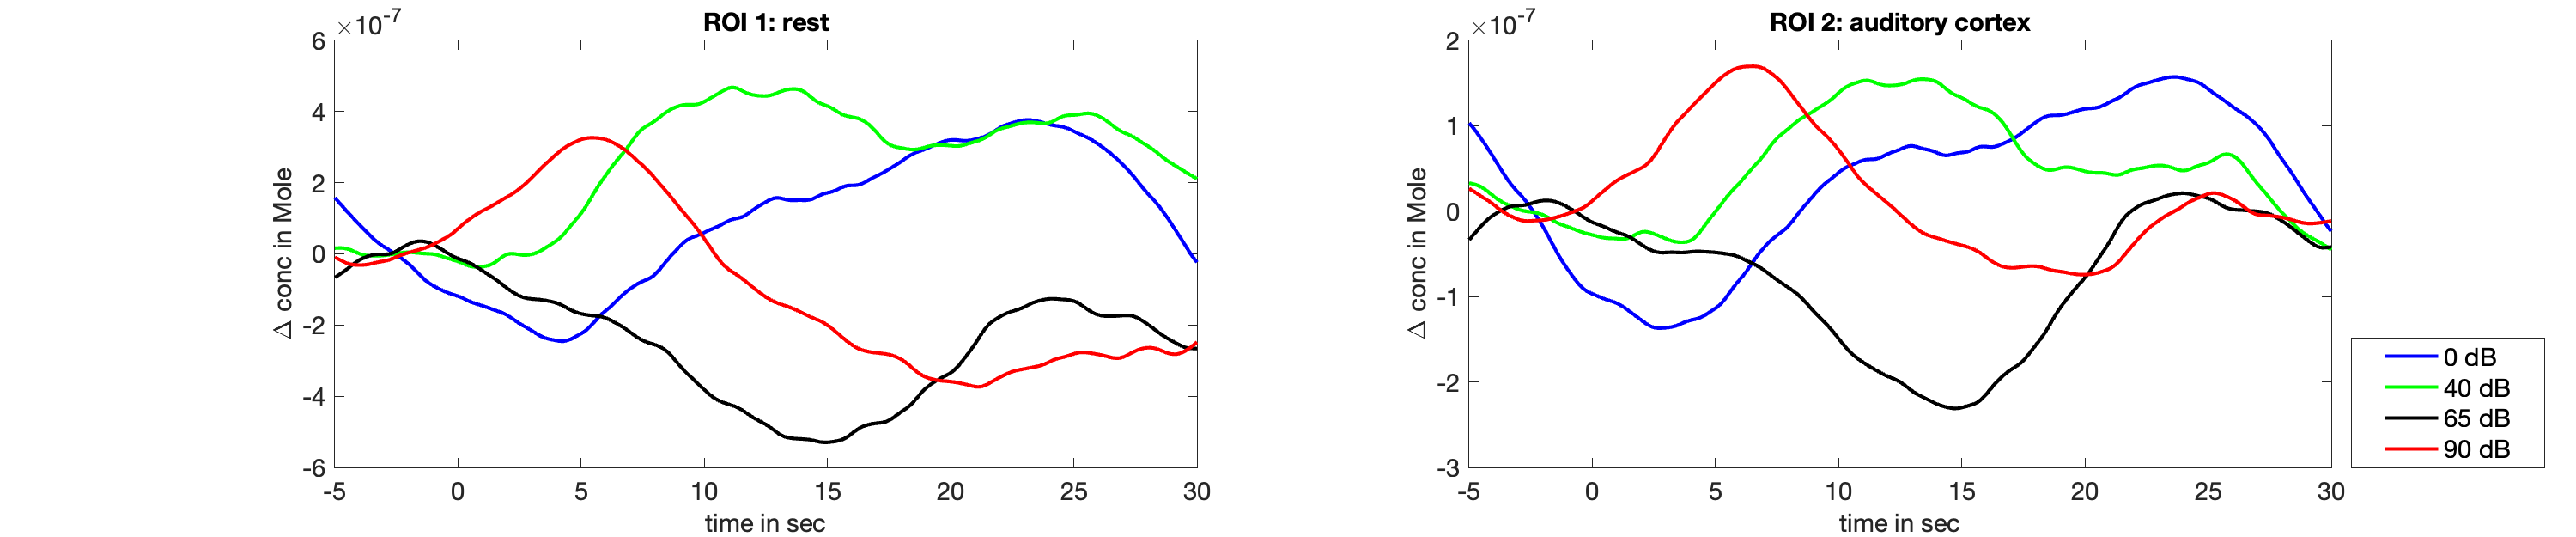
\includegraphics[scale=.29]{bilder/ROI/sub_shelia_s_HbO.png}
  \caption{Measurement from participant  6.}
  \label{fig:somesignal}
\end{figure}


\begin{figure}[H]
  \centering
    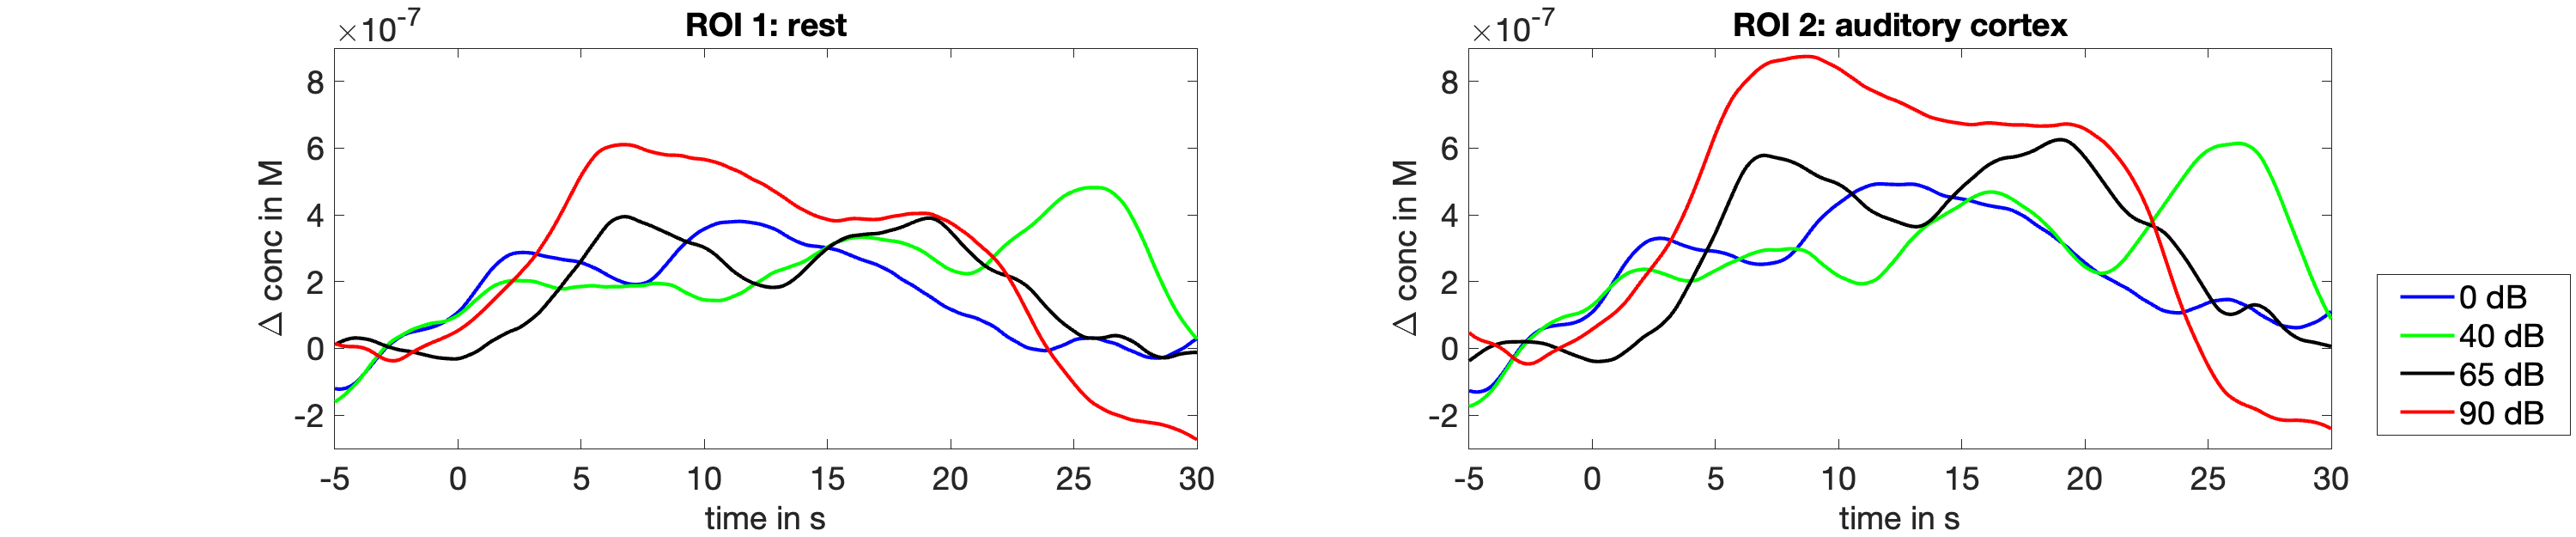
\includegraphics[scale=.29]{bilder/ROI/sub_liao_s_HbO.png}
  \caption{Measurement from participant 7.}
  \label{fig:somesignal}
\end{figure}



\begin{figure}[H]
  \centering
    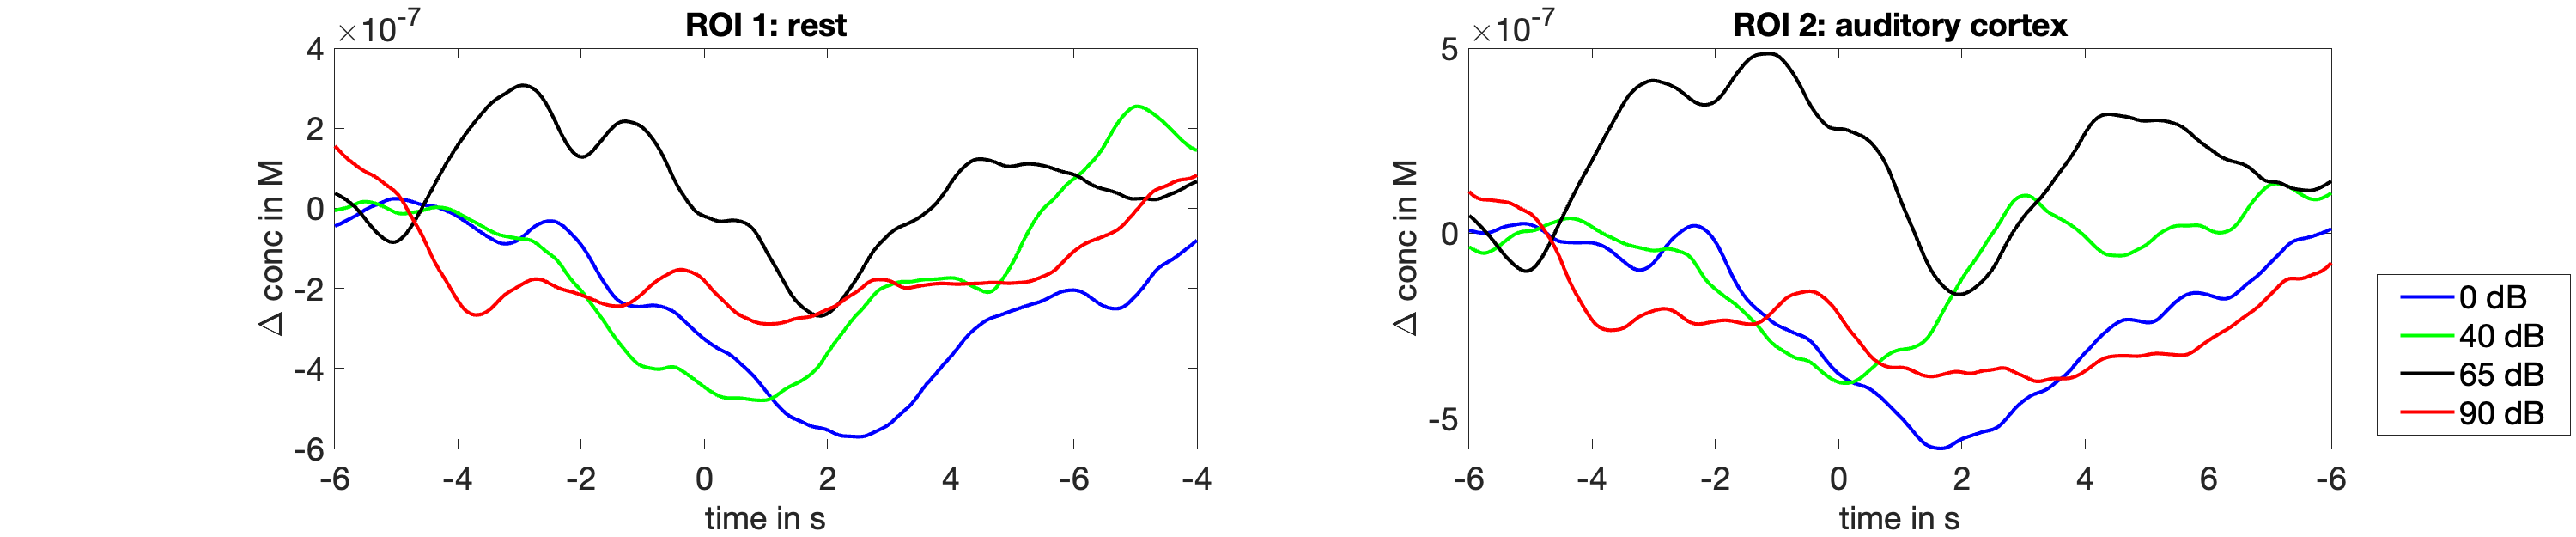
\includegraphics[scale=.29]{bilder/ROI/sub_luca2_s_HbO.png}
  \caption{Measurement from participant 8. Silent comparision.}
  \label{fig:somesignal}
\end{figure}

\newpage

\section {Poor Measurements}
There were also some poor measurements even though the SCI is above the threshold 0.75. For example, in our case of participant 4. One possible reason can be due to the think dark hair of the participant. Light absorption can affect the result greatly.

\begin{figure}[H]
  \centering
    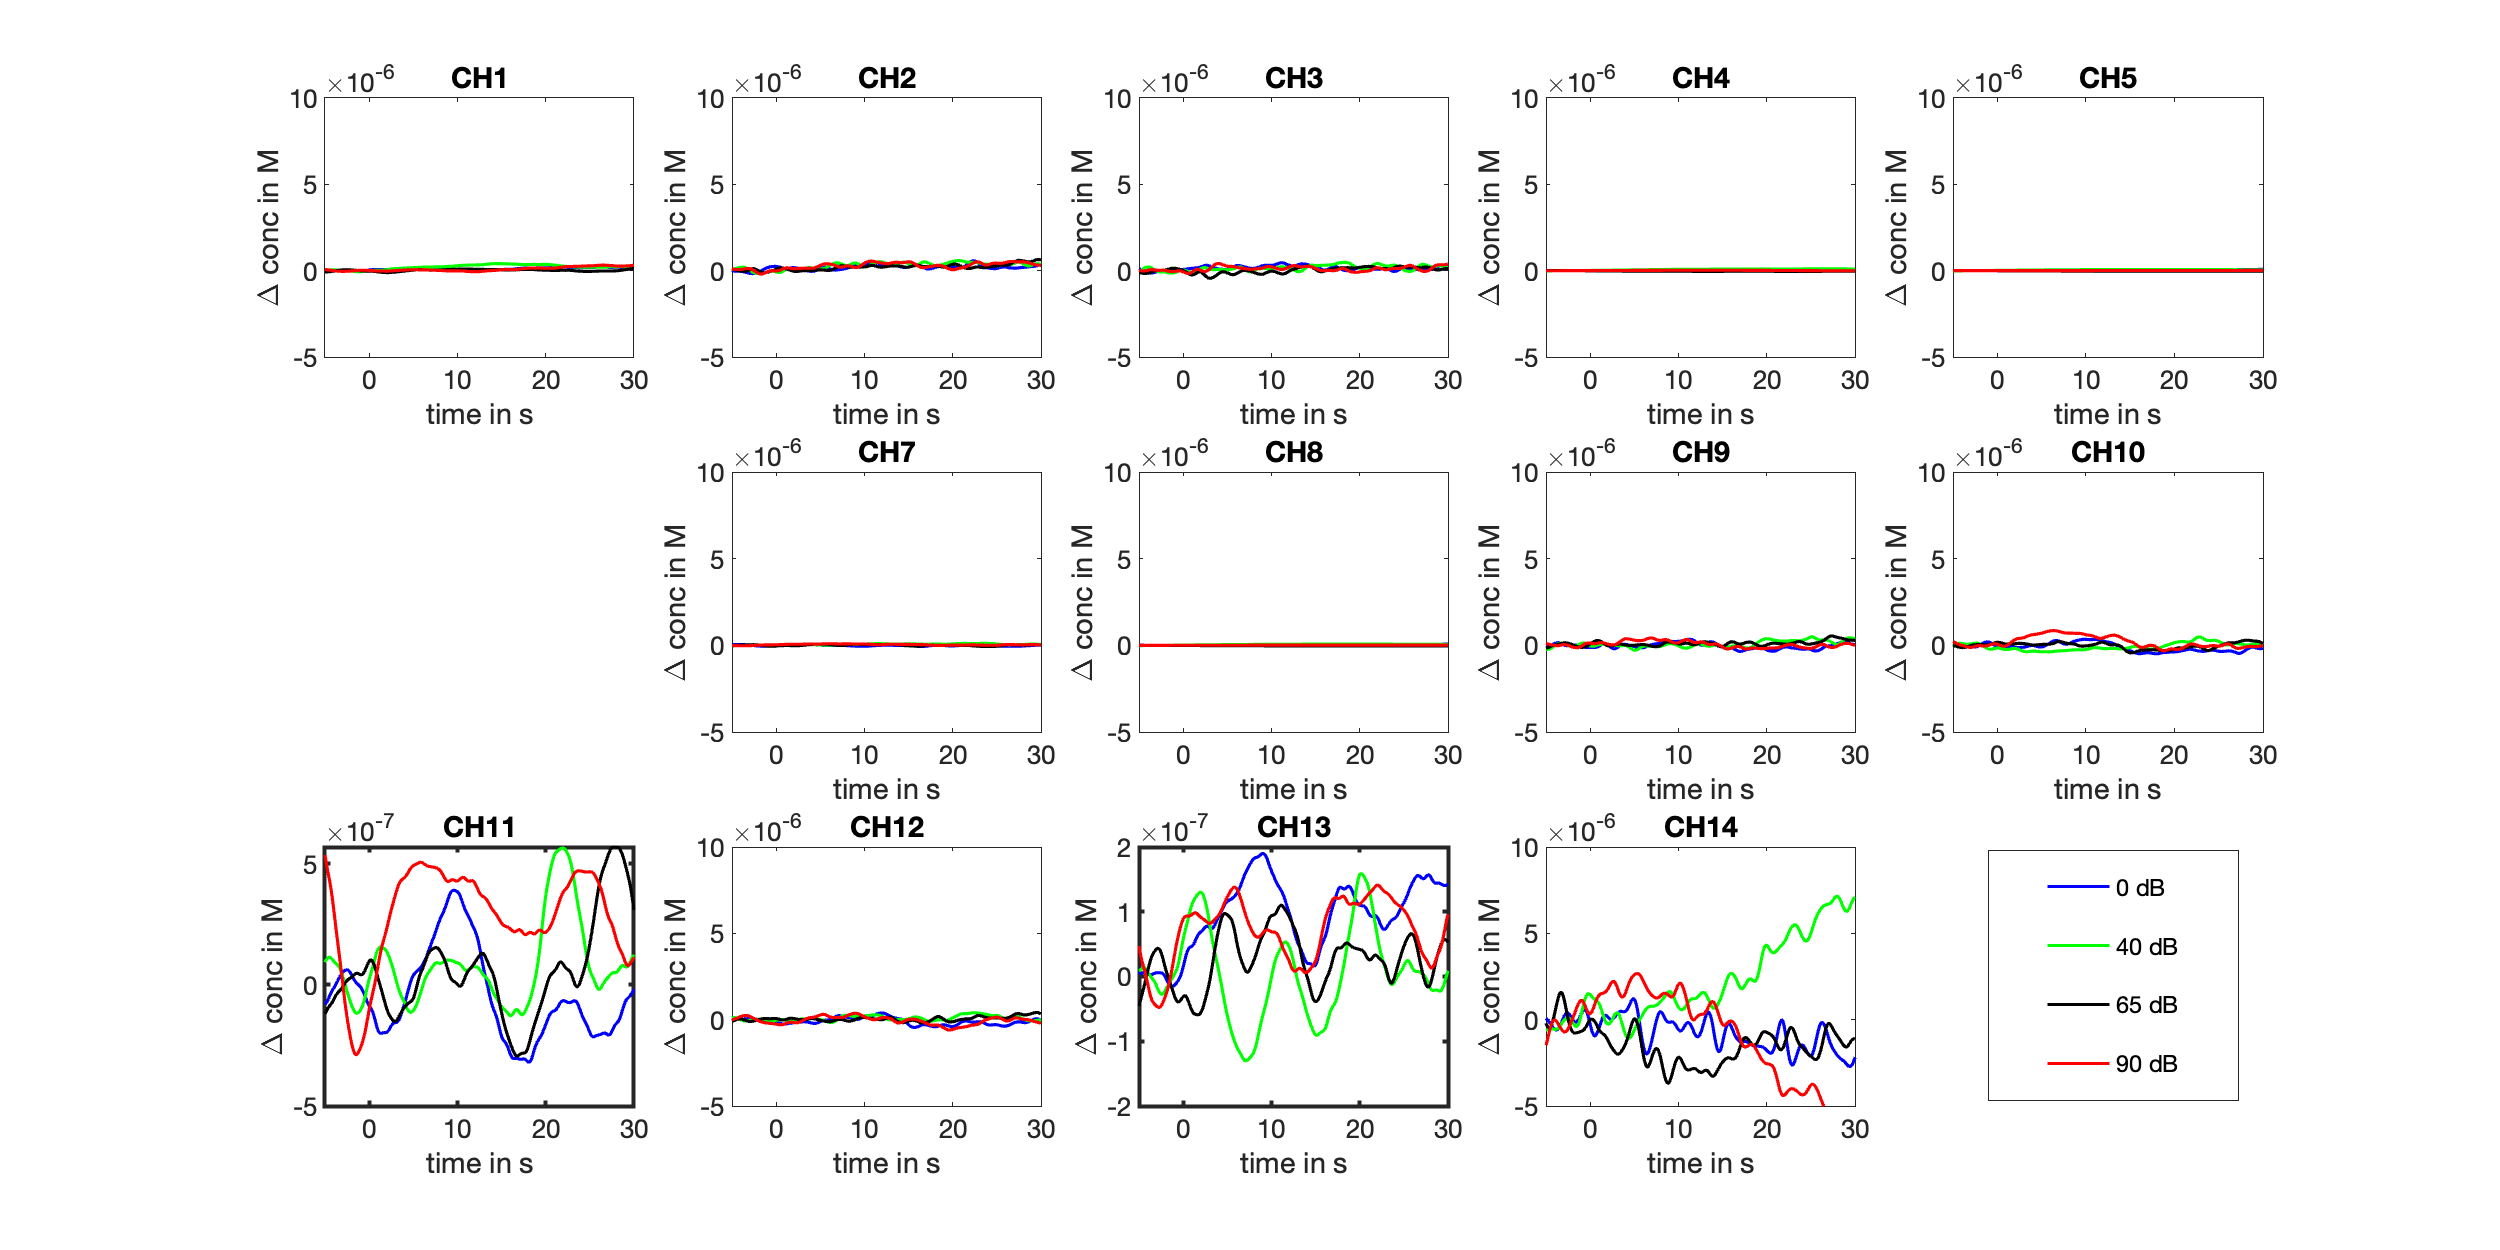
\includegraphics[scale=.35]{bilder/HbO_Mole/sub_lin_s_HbO.png}
  \caption{HbO Measurement from participant 4.}
  \label{fig:somesignal}
\end{figure}


\begin{figure}[H]
  \centering
    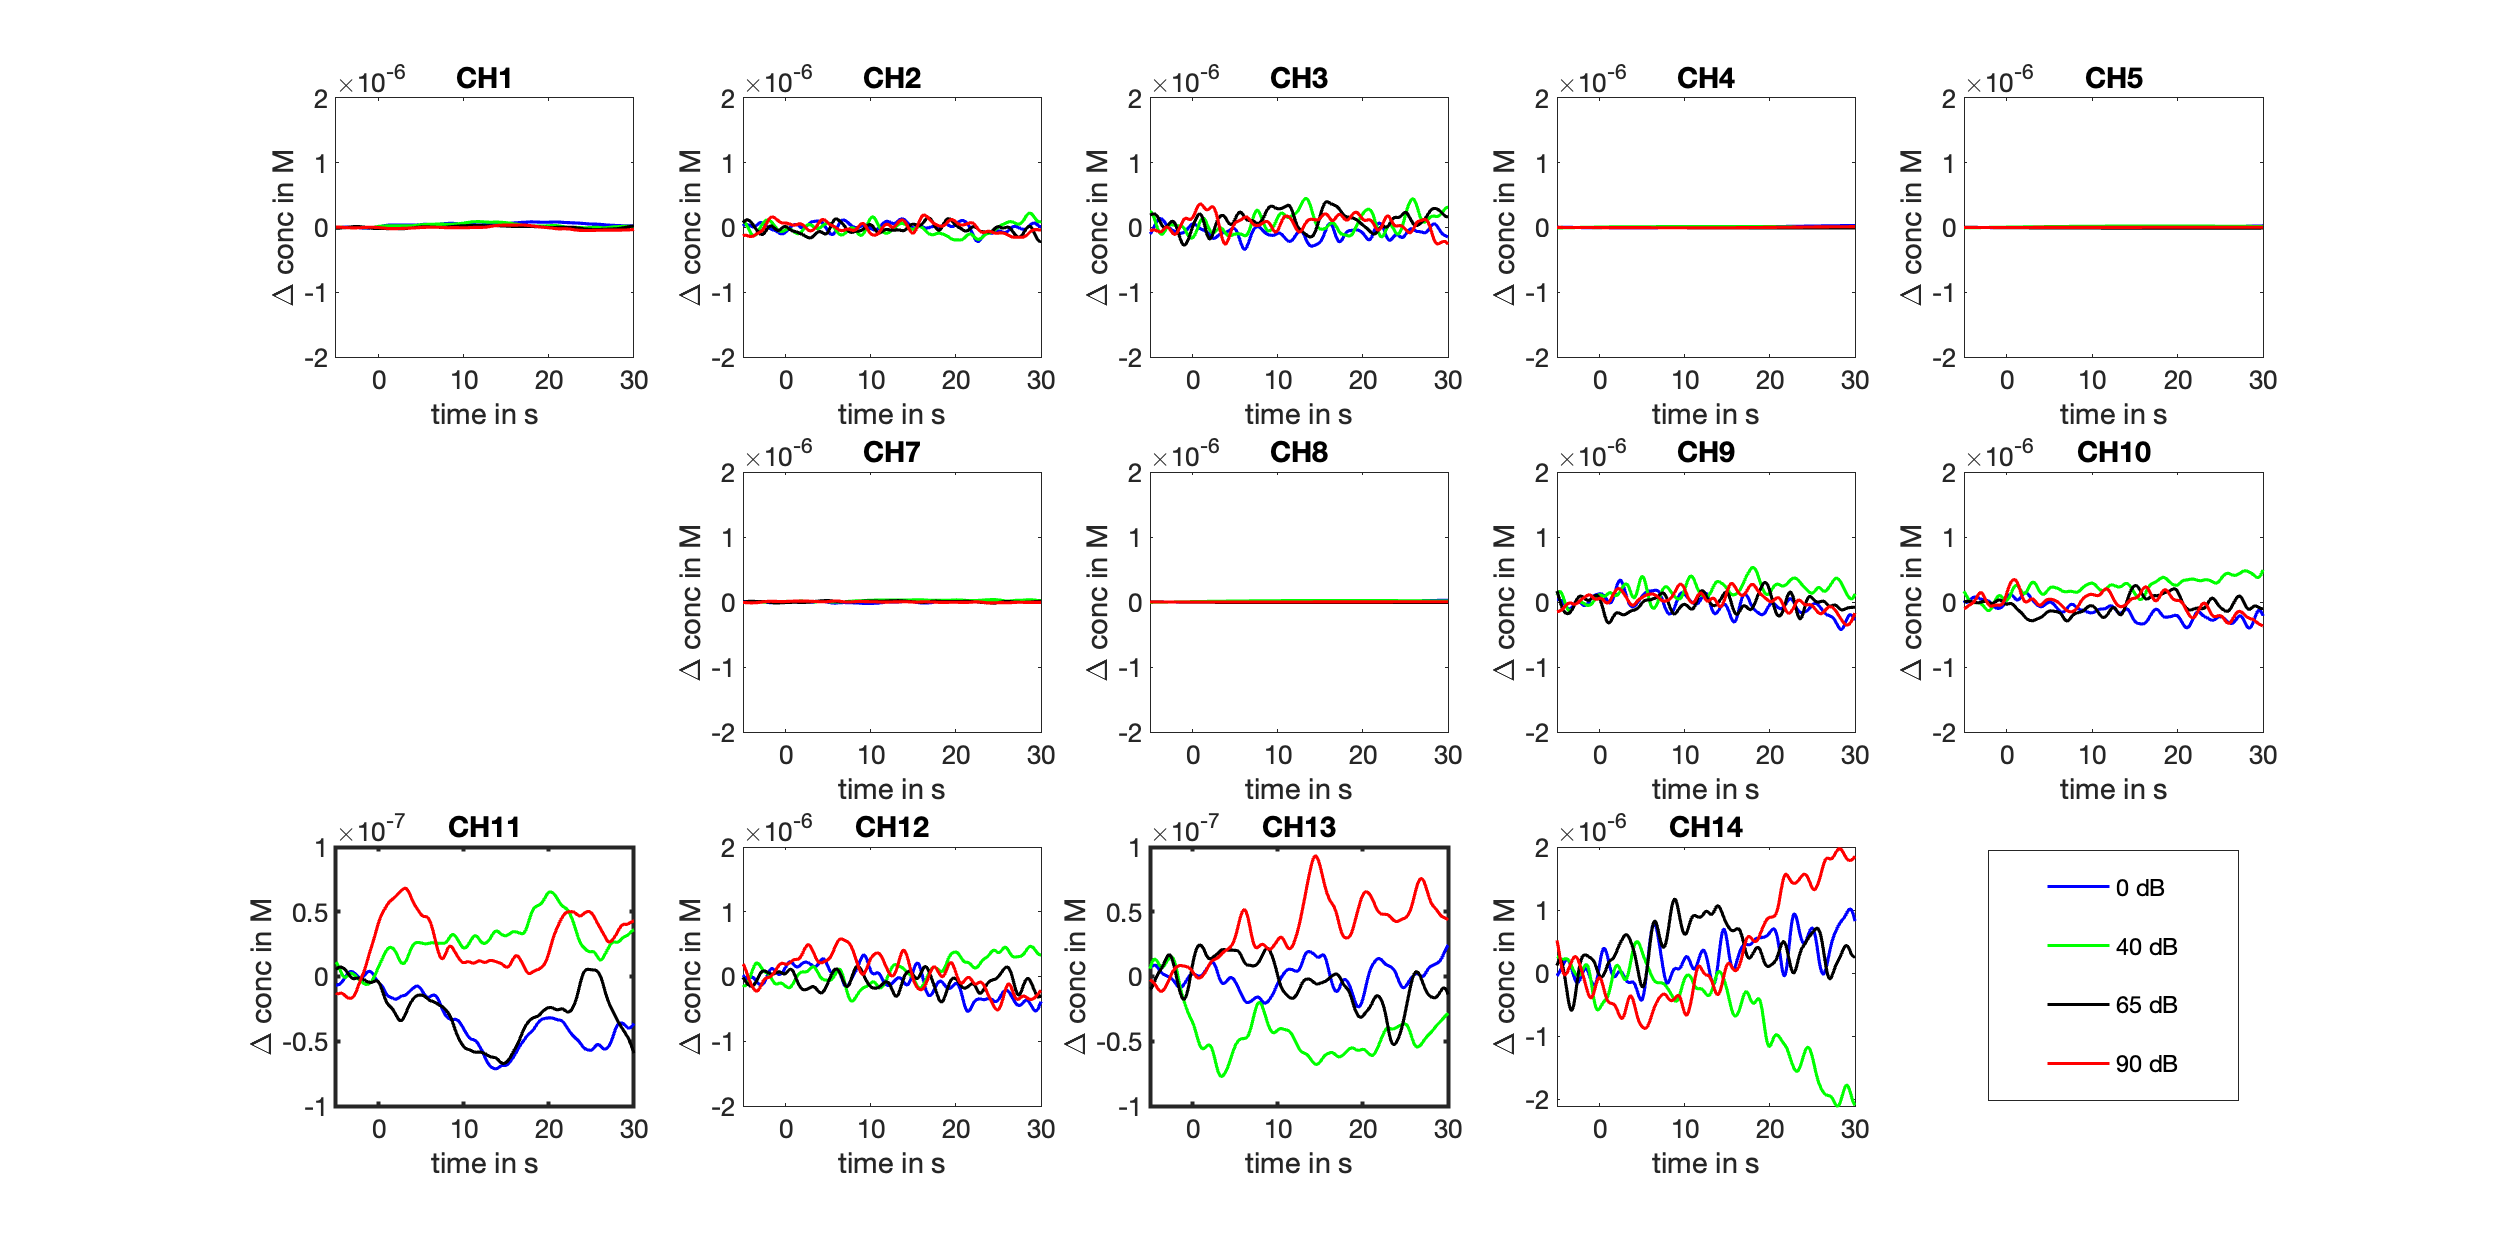
\includegraphics[scale=.35]{bilder/HbR_Mole/sub_lin_s_HbR.png}
  \caption{HbR Measurement from participant 4.}
  \label{fig:somesignal}
\end{figure}

